%!TEX root=TFG-book.tex
	

	
	%	En los mismos términos, F se considera continua en $x_0 \in D \iff \exists \lim_{x \rightarrow x_0} F(x)$ y además:
	%	\[\lim_{x \rightarrow x_0} F(x) = F(x_0)\]
	%	Además, si es continua en todo punto de D, se dice que es continua en D y se escribe $F \in \mathcal{C^0}(D)$.
	%	\end{definition}

\chapter{Métodos directos}

%%En el primer capítulo de este trabajo desarrollaremos los métodos directos de resolución de sistemas de ecuaciones no lineales, como son el método del punto fijo, el método de Newton y los métodos cuasi-Newton. Estos métodos abordan de manera directa el problema planteado mediante métodos numéricos.

Los métodos directos de resolución de sistemas de ecuaciones son aquellos que permiten calcular la solución del sistema en un número finito de pasos. De esta forma, vamos a abordar el problema del cálculo de la solución de forma directa mediante los métodos del punto fijo, el método de Newton y los métodos cuasi-Newton.

Un sistema de ecuaciones no lineales:

$$\begin{cases}
	f_1(x_1,\dots,x_n)  = 0 \\
	f_2(x_1,\dots,x_n)  = 0 \nonumber \\
	...                   \nonumber \\
	f_n(x_1,\dots,x_n)  = 0 \nonumber
\end{cases}$$

donde podemos considerar la función $f_i$ como mapeo del vector $x = (x_1,\dots,x_n)$ del espacio dimensional $\mathbb{R}^n$ en la recta real $\mathbb{R}$. Este sistema también se puede representar como una única función de $\mathbb{R}^n$ en $\mathbb{R}^n$:
\[F(x_1,\dots,x_n) = (f_1(x_1,\dots,x_n),\dots,f_n(x_1,\dots,x_n))\]
Empleando una notación vectorial, de forma que podemos escribir el sistema como:
\[F(x) = 0\]

Nuestro problema será el de encontrar la solución de dicho sistema. 
\section{Puntos fijos para funciones de varias variables}

\begin{definition}
	Se dice que una función $G$ de $D \subset \mathbb{R}^n$ tiene un punto fijo en $p \in D$ si $G(p) = p$.
\end{definition}

	Equivalentemente al problema de encontrar un cero, podemos reescribir el sistema como un problema de punto fijo, que tendrá las mismas soluciones. De esta forma denominamos $G:\mathbb{R}^n \longrightarrow \mathbb{R}^n$, donde $F(x) = G(x) - x = 0$. Para transformar de forma inversa, podemos sumar un término $x$ a ambos lados de la ecuación, o alternativamente despejar el término $x$ si aparece de forma independiente en la ecuación $F(x)$ original. De esta forma, vemos que si la función $G$ tiene un punto fijo, entonces $F$ poseerá un cero en ese mismo punto. \\
% Tomamos D cerrado porque sino tendríamos que definir los puntos que tienen límite como los de D' de su conjunto de acumulación o clausura

%	Recordemos que dada $F: D \subset \mathbb{R}^n \longrightarrow \mathbb{R}^m$, donde su dominio D es un conjunto cerrado, de forma que la función $f$ es contractiva en D, se dice que tiene límite $L \in  \mathbb{R}^m$ en $x_0 \in D$ y se escribe:
%	\[\lim_{x \rightarrow x_0} F(x) = L\]
%	si dado $\epsilon > 0$, existe un $ \delta > 0$ tal que para todo
%	$ x \in D$:
%	 $$0 < \|x-x_0\| < \delta \Rightarrow ||f(x) - L|| < \epsilon $$
%	La existencia de límite es independiente de la norma vectorial que se use. 
	%El valor $\delta$ es independiente de la norma.

%	\begin{definition}
	%	Sea $f: D \subset \mathbb{R}^n \longrightarrow \mathbb{R}$. Se dice que es continua en $x_0 \in D$ siempre que $\exists \lim_{x \rightarrow x_0} f(x)$ y además:
	%	\[\lim_{x \rightarrow x_0} f(x) = f(x_0)\]
	%	Además, si es continua en todo punto de D, se dice que es continua en D y se escribe $f \in \mathcal{C^0}(D)$.	
	%	\end{definition}

%Para poder estudiar de forma sencilla el límite de funciones en varias dimensiones, es más sencillo estudiar el límite para cada una de las componentes:
%
%\begin{proposition}
%	Sea $F: D \subset \mathbb{R}^n \longrightarrow \mathbb{R}^m$ de la forma $F(x) = (f_1(x),...,f_m(x))$, donde $f_i: D \subset \mathbb{R}^n \longrightarrow \mathbb{R}$ , $1 \leq i \leq m$. Entonces el límite:
%	\[\lim_{x \rightarrow x_0} F(x) = L = (L_1,...,L_m) \iff \lim_{x \rightarrow x_0} f_i(x) = L_i \; , \; 1 \leq i \leq m\]
%\end{proposition}

%	\begin{definition}
	
% Introduccion


De esta manera, podemos introducir el método del punto fijo, también denominado método de aproximaciones sucesivas. Éste, dado un valor inicial $x_0$, toma un esquema iterativo que cumple que cada punto $x_i$ es la imagen $G(x_{i+1})$ del punto anterior. Este método nos acerca sucesivamente al valor $x = G(x)$ con una cota de error predeterminada, siempre que $G$ sea continua y que cada $x_i \longrightarrow x$ converjan a un punto fijo. \\


% CTRL + t para comentar
% CTRL + u para descomentar

%\begin{theorem}
%	Sea $f$ una función de $D \subset \mathbb{R}^n$ en $\mathbb{R}$, y $x_0 \in D$. Si existen constantes $\delta > 0$ y $K > 0$, con
%	\[\left| \frac{\partial f(x)}{\partial x_j}  \right| \leq K, j = 1 ,..., n\]
%	siempre que $||x-x_0|| < \delta$ y $x \in D$, entonces $f$ es continua en $x_0$.

%\end{theorem}

 Vamos a ver que siempre se pueden encontrar una solución a la ecuación del punto fijo bajo ciertas condiciones:

\begin{theorem}[Teorema de existencia de punto fijo]
	Sea $$D = \{(x_1,...,x_n) , a_i \leq x_i \leq b_i, \forall i = 1 ,..., n\}$$ para algún conjunto de constantes $a_1$, ..., $a_n$ y $b_1$, ..., $b_n$. Si $G : D \subset \mathbb{R}^n \longrightarrow \mathbb{R}^n$ es una función continua tal que $G(D) \subseteq D$ y es lipschitziana de constante $0<K<1$, entonces la sucesión $\{x_{k}\}_{k \in \mathbb{N}}$ dada por $x_{0} \in D$ y generada por:
	\[x_{k} = G(x_{k-1} )\ \forall k \geq 1\]
	converge en un único punto fijo $p \in D$ y además:
	\[||x_{k} - p|| \leq \frac{K^k}{1-K}||x_{1} - x_{0}|| \]
\end{theorem}

\begin{proof}
	Como $G$ es lipschitziana, tenemos que:
	\begin{align*}
	|| x_{k} - x_{k-1} || & = || G(x_{k-1}) - G(x_{k-2}) || \leq K || x_{k-1} - x_{k-2} || \\
	& \leq K^2|| x_{k-2} -  x_{k-3} || \leq \ldots \leq K^{k-1}|| x_{1} - x_{0} ||
	\end{align*}

	Veamos que $\{x_{k}\}$ es una sucesión de Cauchy. Como $D$ está acotado, podemos tomar un $r > 0$ con $||x_{1} - x_{0}||\leq r(1-K) \leq r$, pues $0 < K < 1$. Tomaremos esta cota únicamente para simplificar el resultado. \\
 	Dado $m>l$, entonces:

	\begin{align*}
	||x_{m}-x_{l}||& \leq ||x_{m} - x_{m-1}|| + ||x_{m-1} - x_{m-2}|| +  \ldots+||x_{l+1} -  x_{l}||\\
	& \leq (K^{m-1} + K^{m-2} + \ldots + K^l) (1-K)r \\
	\end{align*}
	Resolvemos esta serie geométrica y acotamos convenientemente:
	\begin{align*}
	\sum_{i = k-1}^{l} K^{i} = K^{l} \sum_{i = 0}^{m-1-l} K^{i} = K^{l}\frac{1-K^{m-l}}{1-K} < \frac{K^{l}}{1-K}
	\end{align*}
	\begin{align*}
	||x_{m}-x_{l}|| < \frac{K^{l}}{1-K} ||x_{1}-x_{0}|| < K^{l} r
	\end{align*}

	Por lo tanto, como $K<1$, podemos hacer $K^lr$ arbitrariamente pequeño para $l$ suficientemente grande.
	
	Con esto hemos visto que $\{x_{k}\}$ es sucesión de Cauchy, luego converge a un $p$ en el espacio completo $\mathbb{R}^{n}$. Como $D$ es cerrado y $x_{k} \in D$, $\forall$ $k$, $p \in D$.
	
	Por último:
	
	\[||x_{k}-p|| = \lim_{m \to \infty} ||x_{m}-x_{k}|| \leq \frac{K^l}{1-K}||x_{1}-x_{0}||\]
\end{proof}

Vamos a introducir un resultado que nos asegura la convergencia lineal del método del punto fijo:


\begin{theorem}\label{TPF}
	Sea $G : \mathbb{R}^n \to \mathbb{R}^n$ diferenciable y $J_G$ su matriz jacobiana.
	Si $p$ es un punto fijo de $G$ y $||J_G(p)|| = \sigma < 1$, entonces existe un entorno abierto $N$ de $p$ tal que la sucesión definida por $x_{k}=G(x_{k-1})$ con $x_{0}\in N$ converge a $p$.
\end{theorem}
\begin{proof}
	Como $G$ es diferenciable, para todo $\epsilon > 0$ existe un $\delta > 0$ tal que:
	
	\[ ||G(x) - G(p) - J_G(p)(x-p) || \leq \epsilon ||x-p|| \]
	
	cuando $x \in N_\delta(p)=\{x : ||x-p||<\delta\}$. Por lo tanto, para cualquier $x \in N_\delta(p)$:
	
	\[ ||G(x)-G(p)|| \leq ||G(x) - G(p) - J_G(p)(x-p)|| + ||J_G(p)(x-p)|| \leq (\epsilon+\sigma) ||x-p|| \]
	
	Tomando $\epsilon$ suficientemente pequeño, tenemos entonces que para $\alpha=\epsilon+\sigma<1$. Luego si $x_{0} \in N_\delta(p)$, entonces:
	
	\[ ||x_{1}-p|| = ||G(x_{0})-G(p)|| \leq \alpha ||x_{0} - p|| \]
	
	Luego $x_{1} \in N_\delta(p)$. Sigue por inducción que $x_{k} \in N_\delta(p)$ para todo $k$ y además:
	
	\[ ||x_{k}-p|| \leq \alpha ||x_{k-1}-p|| \leq \dots \leq \alpha^k ||x_{0}-p|| \]
	
	Luego $x_{k}$ tiende a $p$ cuando $k \to \infty$.
\end{proof}

\subsection{Algoritmo del punto fijo para sistemas}

Para programar el método podemos seguir las siguientes instrucciones: 


\begin{algorithm}[H]
	\floatname{algorithm}{Algoritmo}
	\caption{Método del punto fijo}
	\textbf{Entrada: } \\
	\hspace*{\algorithmicindent} $f$ \text{ - función real} \\
	\hspace*{\algorithmicindent} $x_0$ \text{ - aproximación inicial} \\
	\hspace*{\algorithmicindent} $TOL$ \text { - tolerancia} \\
	\hspace*{\algorithmicindent} $N$ \text{ - número máximo de iteraciones} \\
	\textbf{Salida:} \\
	\hspace*{\algorithmicindent} $x$ \text{ - punto fijo aproximado de } $f$
	\begin{algorithmic}
		\Procedure {}{}
		\State $x = x_0$
		\For{$k = 1,\dots,N$}
		\State $x = f(x)$
		\If{$\|x\| < TOL$} 
		\State \Return $x$ \Comment{El proceso tuvo éxito}
		\EndIf
		\EndFor
		\State \textbf{imprime} "Número máximo de iteraciones excedido" \Comment{No tuvo éxito}
		\EndProcedure
	\end{algorithmic}
\end{algorithm}

%\begin{algorithm}
%	\caption{Algoritmo del punto fijo}
%	\label{puntoFijo}
%	\begin{algorithmic}[1]
%		\Entrada:
		
		
%		\Procedure{puntoFijo}{$a,b$} \Comment{Busca un valor $x = G(x)$ mediante aproximaciones sucesivas}
%		\State $r\gets a \bmod b$
%		\While{$r\not=0$} \Comment{Si $r$ es cero ya tendríamos la respuesta}
%		\State $a \gets b$
%		\State $b \gets r$
%		\State $r \gets a \bmod b$
%		\EndWhile\label{euclidesfinwhile}
%		\State \textbf{return} $b$\Comment{El M.C.D es $b$}
%		\EndProcedure
%	\end{algorithmic}
%\end{algorithm}

%\begin{itemize}
%\item INPUT número n de ecuaciones ; aproximación inicial $x_0$ 
%\item TOL número máximo de iteraciones N 
%\item Paso 1	Sea k = 1, entonces $x = x_0$ 
%\item Paso 2 Cuando ($k \leq N$) hacer pasos  3 al 6 
%\item Paso 3 Resolver el sistema de punto fijo x = f(x) 
%\item Paso 4 Si $||x|| < TOL $ entonces OUTPUT (x) (El proceso tuvo éxito). STOP 
%\item Paso 5 Sea k = k+1 
%\item Paso 6 OUTPUT ('Número máximo de iteraciones excedido') (El proceso no tuvo éxito). STOP.
%\end{itemize}


Hemos programado el método anterior en SAGE mediante el siguiente código:

\begin{minted}{python}
def MetodoPuntoFijo(f,x0,n):
	x = x0
	for k in [1..n]:
	x = f(*x)
	return x
\end{minted}

O alternativamente, si queremos ver todos los pasos intermedios:
\begin{minted}{python}
def MetodoPuntoFijoIteraciones(f,x0,n):
	x = [x0] + [0]*n
	for k in [1..n]:
	x[k] = f(*x[k-1])
	return x
\end{minted}

\subsection{Ejemplos}

A continuación ilustraremos el método en algunos ejemplos. \\
En primer lugar, consideraremos el método en una dimensión, pues será más sencillo representarlo. \\
Vamos a tomar $cos(x)$ como primer ejemplo. Sabemos que restringido al intervalo $D = [0,\pi]$, el coseno es contractivo, por tanto estamos dentro de las hipótesis del teorema:

\begin{example}
	$$f(x) = \frac{cos(x)}{2}$$
	
	Como sabemos $cos(x)$ es infinitamente diferenciable, tiene un máximo absoluto en cada una de las derivadas dentro del intervalo cerrado D. Por el teorema del valor medio podemos observar que ese máximo nos vale como constante de Lipschitz.
	
	Tomamos $x_0 = 0.5$ y procedemos a aplicar el método.
	Si hacemos 20 iteraciones, obtenemos el valor $x = 0.739006779780813$ como aproximación del punto fijo.
%	
%	Para escribir en SAGE definimos como:
%	\begin{minted}{python}
%		f(x)=(cos(x),)
%		MetodoPuntoFijo(f,(0.5,),20)
%	\end{minted}
Ya que estamos definiendo el método de forma vectorial.\\

Y la gráfica de la función junto a la recta y=x, que cortan en el punto fijo, junto a las líneas verdes que indican cada una de las iteraciones:

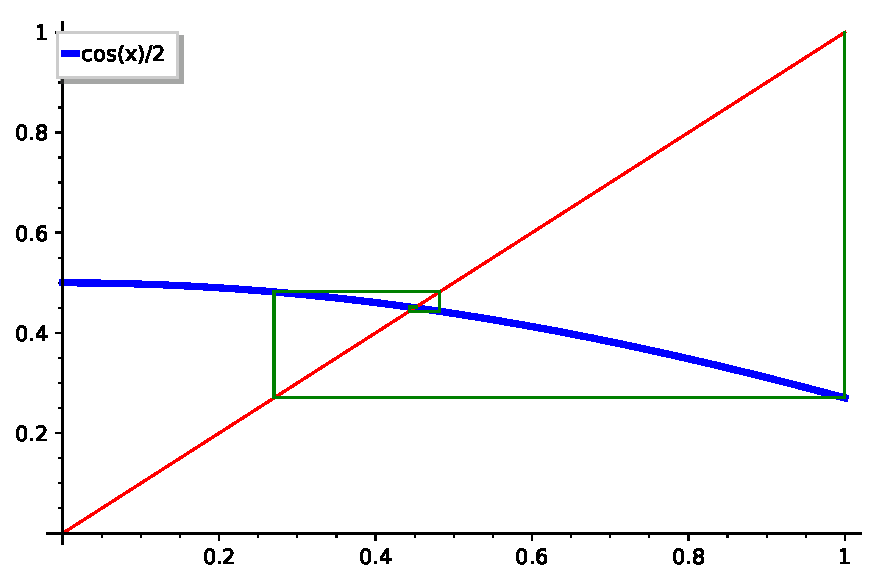
\includegraphics{imagenes/ejemplo1_puntofijo.pdf}
\end{example}

A continuación vamos a introducir un contraejemplo para ver que no todas las funciones contractivas tienen punto fijo:

\begin{example}
$$h(x) = 1+log(1+ exp(x)) $$

Esta función es claramente contractiva, pues si derivamos:
$$|h'(x)| = \frac{e^{x}}{1+e^{x}} < 1$$
Pero para todo $x \in D$, tenemos que $|h(x)-x| > 1$, por lo cual no va a tener un punto fijo.\\

Podemos aplicar el método don 20, 100 y 200 iteraciones. Como podemos observar, los resultados serán $21.1726982050075$, $101.172698206017$ y $201.172698206017$, que no converge a ningún punto, sino que crece indefinidamente. Vamos a verlo gráficamente:


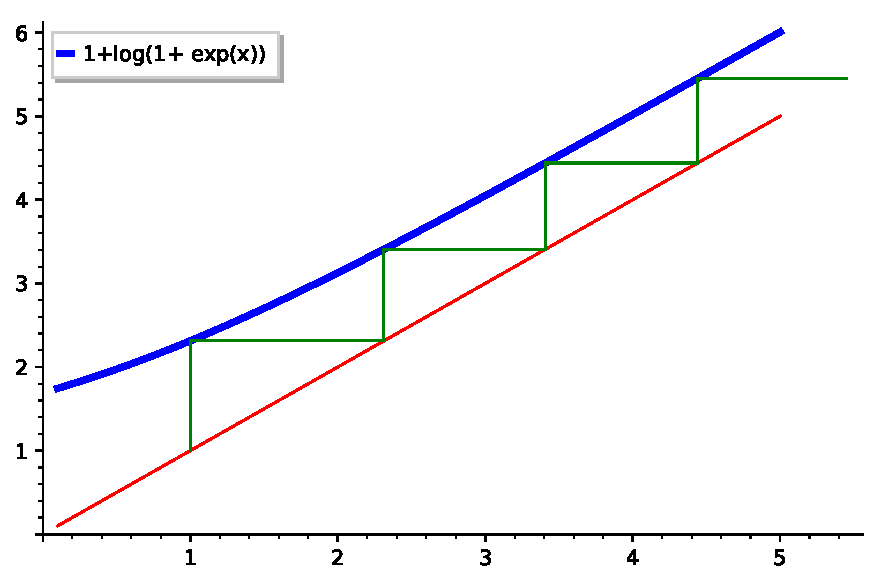
\includegraphics[scale=1]{imagenes/ejemplo2_puntofijo.pdf}

Es claro entonces, pues nuestra función tiene una asíntota en $y=x$. Por eso nunca converge a un punto fijo, pues no se llegan a cortar ambas funciones.


\end{example}

El siguiente ejemplo será bidimensional, para que podamos observar cómo funciona el método en dimensiones superiores:

\begin{example}
	$$m(x,y) = (\frac{1}{e^{x}},\frac{1}{e^{y}})$$
Lo implementamos en SAGE como:
\begin{minted}{python}
	MetodoPuntoFijo(m,(0.5,0.5),10)
\end{minted}

Vemos que con pocas iteraciones el método converge al punto $(0.5669072, 0.5669072)$.

\end{example}

Por último, un ejemplo bidimensional donde no converge el método del Punto Fijo:
\begin{example}
$$
\begin{matrix}
	g_1(x,y) & = x^2+xy-10 \\
	g_2(x,y) & = y + 3xy^2 - 57 \\
	G(x,y)   & = (g_1(x,y),g_2(x,y))
\end{matrix}
$$

Tomamos el punto inicial $(0.5,0.5)$. Si observamos cada iteración podemos ver que esta función no se va aproximando a ningún punto fijo:

\begin{minted}{python}
[(0.500000000000000, 0.500000000000000),
(-9.50000000000000, -56.1250000000000),
(613.437500000000, -89888.5703125000),
(-5.47647242846680e7, 1.48696422300132e13),
(-8.14328857763300e20, -3.63264701075255e34),
(2.95816929092346e55, -3.22379544959185e90),
(-9.53653269920141e145, 9.22314921617083e236),
(-8.79568640896269e382, -2.43371784625526e620),
(2.14062189835574e1003, -1.56290091483395e1624),
(-3.34557992325377e2627, 1.56864297681102e4252),
(-5.24802044997198e6879, -2.46968112630275e11132)]
\end{minted}

	
\end{example}
                                           
%\subsection{Aceleración de la convergencia}
%
%Una forma de acelerar la convergencia en la fórmula del punto fijo es usar la última estimación $x_1^{(k)}$,...,$x_{i-1}^{(k)}$, en lugar de $x_1^{(k-1)}$,...,$x_{i-1}^{(k-1)}$ para computar $x_i^{(k)}$ como lo haríamos en el método de Gauss-Seidel de sistemas lineales.

\subsection{Importancia del método}

La gran importancia del Teorema del Punto Fijo deriva de varios factores. Primero de la existencia y unicidad de solución; De la posibilidad de hallar un error a priori y a posteriori; De ser un método convergente iterativo donde podemos conocer la velocidad de convergencia; Y por último de la estabilidad del método, ya que un cambio en el punto inicial no varía el límite de iteraciones.

\section{Método de Newton}

El método de Newton, también conocido como método de Newton-Raphson, busca la aproximación de raíces de funciones desde una conjetura inicial. \\
Este algoritmo, dada la estimación inicial del cero de cierta función $f$, dibuja la tangente a la curva en dicho punto. Cuando la tangente cruza el eje X obtendremos una nueva estimación de la raíz.\\
Veremos que este método tiene una mayor velocidad de convergencia que el método anterior, pero también requiere de ciertas condiciones locales para asegurarla que antes no requeríamos. Si el cero se encuentra cerca de un punto de inflexión, el método puede no converger, pues la tangente $f'(x)$ a la curva en dicho punto podría ser paralela al eje X y no podríamos estimar un nuevo valor del cero.\\

Consideramos el sistema $$F(x)=0$$ donde $F: D \subset \mathbb{R}^{n} \longrightarrow \mathbb{R}^n$ es una función de clase $\mathcal{C}^{2}$ y $p \in D$ es solución, es decir $F(p) = 0$.
Vamos a transformarlo en un problema de punto fijo $$G(x) = x$$ con G una función de la forma:
\[G(x) = x - A(x)^{-1} F(x)\]
descritos en el apartado anterior, donde cada $x_{i} \in A(x) \subset M_{n}$. El objetivo será elegir A(x) de modo que se verifique el teorema \ref{TPF}, que asegura una convergencia lineal del método del punto fijo.\\
%En esta sección vamos a escribir $G$ como una serie de Taylor en n variables alrededor del punto $p$.

\subsection{Matriz Jacobiana}

Supongamos que nuestra matriz $A(x) \in \mathbf{M}_n$ es matriz cuadrada de valores de $\mathbb{R}^n$ en $\mathbb{R}^n$, que además es no singular cerca de la solución $p$ de $F(x) = 0$. Si llamamos $b_{ij}(x)$ a los elementos de $A(x)^{-1}$, para $G(x) = x - A(x)^{-1}F(x)$, tenemos $g_i = x_i - \sum_{j=1}^{n} b_{ij}(x)f_j(x)$. Así:
\[\frac{\partial g_{i}}{\partial x_{k}}(\mathbf{x})=\left\{\begin{array}{ll}
	1-\sum_{j=1}^{n}\left(b_{i j}(\mathbf{x}) \frac{\partial f_{j}}{\partial x_{k}}(\mathbf{x})+\frac{\partial b_{i j}}{\partial x_{k}}(\mathbf{x}) f_{j}(\mathbf{x})\right), & \text { si } i=k ,\\
	-\sum_{j=1}^{n}\left(b_{i j}(\mathbf{x}) \frac{\partial f_{j}}{\partial x_{k}}(\mathbf{x})+\frac{\partial b_{i j}}{\partial x_{k}}(\mathbf{x}) f_{j}(\mathbf{x})\right), & \text { si } i \neq k .
\end{array}\right.\]

\begin{definition}[Matriz Jacobiana]
	Dada una función $f: \mathbb{R}^n \longrightarrow \mathbb{R}^m$, su matriz jacobiana es la matriz de orden $m x n$  
\[J(\mathbf{x})=\left[\begin{array}{cccc}
	\frac{\partial f_{1}}{\partial x_{1}}(\mathbf{x}) & \frac{\partial f_{1}}{\partial x_{2}}(\mathbf{x}) & \cdots & \frac{\partial f_{1}}{\partial x_{n}}(\mathbf{x}) \\
	\frac{\partial f_{2}}{\partial x_{1}}(\mathbf{x}) & \frac{\partial f_{2}}{\partial x_{2}}(\mathbf{x}) & \cdots & \frac{\partial f_{2}}{\partial x_{n}}(\mathbf{x}) \\
	\vdots & \vdots & & \vdots \\
	\frac{\partial f_{n}}{\partial x_{1}}(\mathbf{x}) & \frac{\partial f_{n}}{\partial x_{2}}(\mathbf{x}) & \cdots & \frac{\partial f_{n}}{\partial x_{n}}(\mathbf{x})
\end{array}\right]\]
\end{definition}

Para aplicar el teorema anterior, impondremos que $\frac{\partial g_i(p)}{\partial x_k} = 0, \forall i \leq 1, \forall k \leq 1$. Entonces cuando $i = k$ tenemos:
\[1=\sum_{j=1}^{n} b_{i j}(\mathbf{p}) \frac{\partial f_{j}}{\partial x_{i}}(\mathbf{p})\]
Y cuando $k \neq i$:
\[\sum_{j=1}^{n} b_{i j}(\mathbf{p}) \frac{\partial f_{j}}{\partial x_{k}}(\mathbf{p})=0\]

Tenemos la matriz jacobiana $J(f) = \Big(\frac{\partial f_i}{\partial x_j} \Big)_{1 \leq i,j \leq n} $.

Imponiendo las condiciones para $k = i$ y para $k \neq i$, obtenemos:
\[A(p)^{-1}J(p) = Id \Rightarrow A(p) = J(p)\]

Entonces podemos decir que una opción para aproximar A(x) puede ser la matriz Jacobiana.

El método de Newton para sistemas no lineales quedaría como:
\[\mathbf{x}_{k}=\mathbf{G}\left(\mathbf{x}_{k-1}\right)=\mathbf{x}_{k-1}-J\left(\mathbf{x}_{k-1}\right)^{-1} \mathbf{F}\left(\mathbf{x}_{k-1}\right)\]

Estudiemos la convergencia de este método. Para ello, nos será útil el siguiente lema:

\begin{lemma}
Sea $F : \mathbb{R}^n \to \mathbb{R}^n$ diferenciable y sea $J$ su matriz jacobiana. Si $J$ es lipschitziana de constante $\gamma$  en un conjunto convexo $D$, entonces para todo $x,y \in D$:
\[ || F(y)-F(x)-J(x)(y-x) || \leq \frac{1}{2} \gamma ||x-y||^2 \]
\end{lemma}
\begin{proof}
Obsérvese que $F(y)-F(x) = \int_0^1 J(x + t(y-x))(y-x) dt$. Para esto basta demostrarlo coordenada por coordenada:

\begin{equation}\label{jacobiana-lipschitz} f_i(y)-f_i(x) = \int_0^1 \sum_{j=1}^n \frac{\partial}{\partial x_j} f_i(x + t(y-x))(y_j-x_j)\end{equation}

Efectivamente, definiendo $g_i(t) = f_i(x+t(y-x))$ se tiene que por el teorema fundamental del cálculo que:

\[ f_i(y)-f_i(x) = g_i(1) - g_i(0) = \int_0^1 g_i'(t) dt \]

Por otro lado:

\[ g_i'(t) = \sum_{j=1}^n \frac{\partial}{\partial x_j} f_i(x + t(y-x))(y_j-x_j) \]

de donde se deduce la ecuación \eqref{jacobiana-lipschitz}. Por lo tanto:

\begin{align*}||F(y)-F(x) - J(x)(y-x)|| & = ||\int_0^1 J(x + t(y-x))(y-x) dt- J(x)(y-x)||\\
& \leq \int_0^1 ||J(x + t(y-x))(y-x)- J(x)(y-x)||\\
& = \int_0^1 ||(J(x + t(y-x))- J(x))||\ ||(y-x)|| dt\\
& \leq \int_0^1 \gamma ||(x + t(y-x)) - x)||\ ||(y-x)|| dt\\
& = \gamma \int_0^1 t\ dt ||x-y||^2\\
& = \frac{1}{2} \gamma ||x-y||^2
\end{align*}
\end{proof}

Gracias a este lema y al teorema \ref{TPF}, podemos demostrar el siguiente teorema sobre la convergencia local del método de Newton:

\begin{theorem}\label{convergencia-local-newton}
Sea $F : \mathbb{R}^n \to \mathbb{R}^n$ tal que:

\begin{itemize}
	\item Hay una solución $p$ de la ecuación $F(x)=0$.
	\item $F$ es continua y diferenciable en un entorno abierto de $p$.
	\item El jacobiano $J$ de $F$ es continuo y no singular en un entorno de $p$
	\item El jacobiano $J$ es lipschitziano de constante $\gamma$.
\end{itemize}

Entonces el método de Newton dado por:

\[ x_{k} = x_{k-1} - (J(x_{k-1}))^{-1}F(x_{k-1}) \]

converge cuadráticamente a $p$.
\end{theorem}
\begin{proof}
Tomemos la función $G(x) = x - (J(x))^{-1}F(x)$. $G$ está bien definida y es diferenciable en un entorno abierto de $p$.
Como el jacobiano $J_G(p) = I - (J(p))^{-1}J_F(p) = 0$, tenemos por el teorema \ref{TPF} que en un entorno de $p$, la sucesión $x_{k}$ converge $p$ por ser punto fijo de $G$.

Además, como $J$ es lipschitziana se deduce por el anterior lema que:

$$ || F(y)-F(x)-J(x)(y-x) || \leq \frac{1}{2} \gamma ||x-y||^2 $$

Por otro lado, de la continuidad y no singularidad de $J_F$ se puede deducir que en un entorno de $p$, $||(J(x))^{-1}|| \leq M$ para cierto $M > 0$. Por lo tanto:

\begin{align*}||G(x)-G(p)|| & = || x-(J(x))^{-1}F(x)-p||\\
& = ||(J(x))^{-1}||\ || J(x)x-F(x)-J_F(x)p||\\
& \leq M || F(p) - F(x) - J(x)(p-x)||\\
& \leq \frac{\gamma M}{2} ||x-p||^2
\end{align*}

Lo que prueba la convergencia cuadrática.
\end{proof}

De este método podemos esperar convergencia cuadrática, suponiendo que el valor inicial que nos dan es lo suficientemente cercano a la solución y que además existe la matriz inversa $J(p)^{-1}$. \\
Lo negativo de este método radica en la necesidad de calcular e invertir la matriz $J$ a cada paso que damos, pero en la práctica podemos evitar calcular la inversa separando la operación en dos pasos:
\begin{enumerate}
	\item Buscamos un vector $v$ que cumpla $J(x_{k-1})v = -F(x_{k-1})$.
	\item $x_{k} = x_{k-1} + v$.
\end{enumerate}
\subsection{Algoritmo de Newton para sistemas}

Si queremos programar el sistema $F(x) = 0$ dada una aproximación inicial, podemos hacerlo siguiendo las siguientes instrucciones: \\

\begin{algorithm}[H]
	\floatname{algorithm}{Algoritmo}
	\caption{Método de Newton}
	\textbf{Entrada: } \\
	\hspace*{\algorithmicindent} $f$ \text{ - función real} \\
	\hspace*{\algorithmicindent} $x_0$ \text{ - aproximación inicial} \\
%	\hspace*{\algorithmicindent} $TOL$ \text { - tolerancia} \\
	\hspace*{\algorithmicindent} $N$ \text{ - número máximo de iteraciones} \\
	\textbf{Salida:} \\
	\hspace*{\algorithmicindent} $x$ \text{ - lista de aproximaciones al cero de } $f$
	\begin{algorithmic}
		\Procedure {}{}
		\State $x = x_0$
		\State $J = \Big(\frac{\partial f_i}{\partial x_j}\Big)_{1 \leq i , j \leq n}$ \Comment{Matriz Jacobiana de f}
		\For{$k = 1,\dots,N$}
		\State $y = J(x)^{-1} (-F(x))$
		\State $x = x + y$
		%\If{$\|x\| < TOL$} 
		\State \Return $(x_1, \dots , x_N)$ \Comment{El proceso tuvo éxito}
%		\EndIf
		\EndFor
%		\State \textbf{imprime} "Número máximo de iteraciones excedido" \Comment{No tuvo éxito}
		\EndProcedure
	\end{algorithmic}
\end{algorithm}

%\begin{itemize}
%\item INPUT número $n$ de ecuaciones e incógnitas; aproximación inicial $\mathbf{x}=\left(x_{1}, \ldots, x_{n}\right)^{t}$ tolerancia $T O L ;$ número máximo de iteraciones $N$. 
%\item OUTPUT $\quad$ solución aproximada $\mathbf{x}=\left(x_{1}, \ldots, x_{n}\right)^{t}$ ó un mensaje que indique que el número de iteraciones se ha excedido.
%\item Paso $1 \quad$ Sea $k=1$
%\item Paso 2 $\quad$ Cuando $(k \leq N)$ hacer pasos $3-7$
%\item Paso 3 $\quad$ Calcular $\mathbf{F}(\mathbf{x})$ y $J(\mathbf{x}),$ donde $J(\mathbf{x})_{i, j}=\left(\partial f_{i}(\mathbf{x}) / \partial x_{j}\right)$ para $1 \leq i, j \leq n$
%\item Paso $4 \quad$ Resolver el sistema lineal $n \times n$ con $J(\mathbf{x}) \mathbf{y}=-\mathbf{F}(\mathbf{x})$
%\item Paso $5 \quad$ Sea $\mathbf{x}=\mathbf{x}+\mathbf{y}$
%\item Paso $6 \quad$ If $\|\mathbf{y}\|<T O L$ entonces OUTPUT $(\mathbf{x})$ (EL proceso tuvo éxito.) STOP.
%\item Paso $7 \quad$ Set $k=k+1$
%\item Paso $8 \quad$ OUTPUT ('Número máximo de iteraciones excedido'); (El proceso no tuvo éxito.) STOP.
%\end{itemize}


\begin{minted}{python}
	def NewtonMetodo(f, x0, n):
		xk = x0
		J = jacobian(f, f[0].arguments())
		for k in [1..n]:
			yk = J(*xk).solve_right(-f(*xk))
			xk = [xki.n()+yki.n() for (xki,yki) in zip(xk,yk)]
		print(xk)
\end{minted}

\subsection{Ejemplos}

\begin{example}
	
Comenzamos con un ejemplo de una variable:
$$f(x) = x^3 - 3x - 5$$
Calculamos la derivada y aplicamos la fórmula del método de Newton como hemos visto:
$$x_{k+1} = x_{k} - \frac{ x_k^3 - 3x_k - 5}{3x_k^2-3}$$

La derivada no se anula en el intervalo abierto $(1.5, 3)$.
Además, $f(1.5)<0$ y $f(3)>0$, luego por continuidad de $f$, existe una solución de $f$ en dicho intervalo.
En consecuencia del teorema \ref{convergencia-local-newton} el método de Newton converge partiendo de un $x_0$ en el intervalo.

De esta forma, obtenemos las siguientes iteraciones, partiendo de $x_0 = 2$:
\begin{equation}
	\begin{matrix}
		&2.0000000000000000000 \\
		&2.3333333333333333333 \\
		&2.2805555555555555556 \\
		&2.2790200679500897523 \\
		&2.2790187861674863832 \\
		&2.2790187861665935795 \\
	\end{matrix}
\end{equation}

Así, después de 5 iteraciones obtenemos el valor $x = 2.279018$ como aproximación de la solución.
\begin{center}
	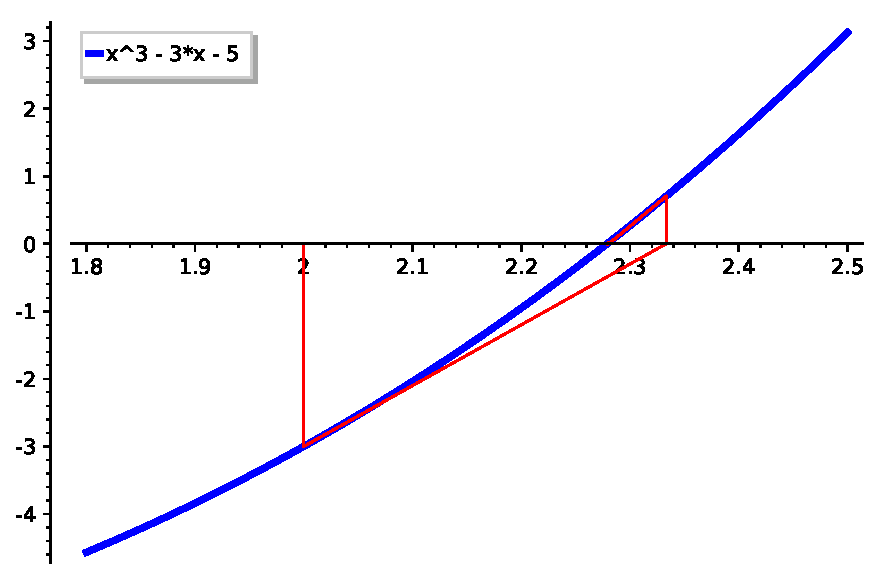
\includegraphics[scale=1]{imagenes/ejemplo1_newton.pdf}
\end{center}


\end{example}

\begin{example}
La convergencia cuadrática del método para una raíz simple indica que el error se eleva al cuadrado en cada iteración asintóticamente. Es decir, que el número de dígitos correctos en la aproximación se duplica en cada iteración. Para una raíz múltiple, el método solo será linealmente convergente. Veamos con este ejemplo: $$f(x) = x^2 - 2x + 1$$
El método será entonces: $$x_{k+1} = x_{k} - \frac{ x_k^2 -2x_k + 1}{2x_k-2}$$
La derivada se anula en $x = 1$. No cumple las condiciones del teorema de convergencia cuadrática. Además, podemos observar que es un mínimo de la función.

Obtenemos las siguientes iteraciones, partiendo de $x_0 = 2$:
	\begin{minted}{python}
		2.00000000000000
		1.50000000000000
		1.25000000000000
		1.12500000000000
		1.06250000000000
		1.03125000000000
		1.01562500000000
		1.00781250000000
		1.00390625000000
		1.00195312500000
		1.00097656250000
	\end{minted}

\begin{center}
	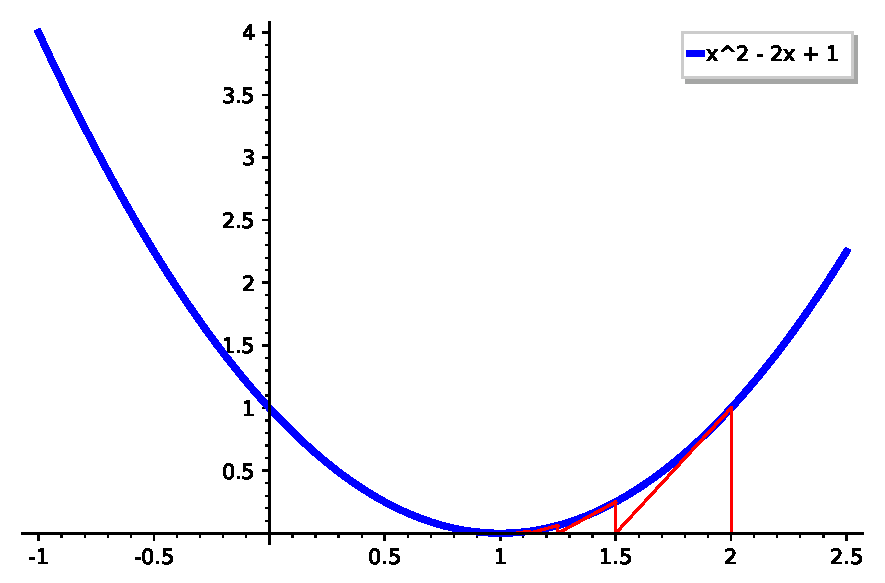
\includegraphics[scale=1]{imagenes/ejemplo2_newton.pdf}
\end{center}
	
\end{example}

\begin{example}

Ahora veamos un ejemplo con 3 variables:

\begin{align*}
	f_1(x,y,z) &= 3x - cos(yz) - \frac{1}{2} \\
	f_2(x,y,z) &= x^2 - 81(y+0.1)^2 + sin(z) + 1.06\\
	f_3(x,y,z) &= exp(-xy) + 20z + \frac{10\pi-3}{3}
\end{align*}

Denotamos $F(x,y,z) = (f_1(x,y,z),f_2(x,y,z),f_3(x,y,z))$.
Hacemos el jacobiano y obtenemos $J_F =(\frac{\partial f_i}{\partial x_j})_{ij}$:
$$
	J_F = 
	\begin{pmatrix}
	3 & z sin(yz) & y sin(yz) \\
	2 & -162y-16.2 & cos(z) \\
	-ye^{-xy} & -xe^{-xy} & 20
	\end{pmatrix}
$$
Encontrar una buena aproximación inicial no es tarea fácil, pues queremos evitar puntos donde el jacobiano sea singular para que el método converja.
Sin embargo, encontrar dónde $J_F$ es singular es también una tarea computacionalmente costosa.\\
En general, un procedimiento habitual es encontrar una aproximación lineal o cuadrática del problema y tomar como estimación inicial una solución del problema simplificado.
Para este ejemplo, partiremos del punto $x_0 = (0.1,0.1,-0.1)$ y obtenemos las siguientes iteraciones:
\begin{minted}{python}
	[0.1,0.1,-0.1]
	[0.499869672926428, 0.0194668485374181, -0.521520471935831]
	[0.500014240164219, 0.00158859137029389, -0.523556964347638]
	[0.500000113467834, 0.0000124447833215538, -0.523598450072889]
	[0.500000000007076, 7.75785730794398e-10, -0.523598775578007]
	[0.500000000000000, 0.000000000000000, -0.523598775598299]
\end{minted}

Por tanto, obtenemos la aproximación a la solución $(0.5, 0, -0.52359)$.

%	\begin{minted}{python}
%		# Ejemplo Newton no lineal
%		#x = var('x')
%		#y = var('y')
%		#z = var('z')
%		f1(x,y,z) = 3*x - cos(y*z) - 1/2
%		f2(x,y,z) = x^2 - 81*(y+0.1)^2 + sin(z) + 1.06
%		f3(x,y,z) = exp(-x*y) + 20*z + (10*pi-3)/3
%		show(f1,f2,f3)
%		
%		F(x,y,z) = (f1(x,y,z),f2(x,y,z),f3(x,y,z))
%		show(F)
%		
%		jacobian(F, F[0].arguments())
%		
%		F(x,y,z).diff(x,1)
%		
%		t = var('t')
%		Fx = F.diff(x)
%		Fy = F.diff(y)
%		Fz = F.diff(z)
%		show(Fx,Fy,Fz)
%		
%		dFx = vector(Fx)
%		dFy = vector(Fy)
%		dFz = vector(Fz)
%		show(dFx,dFy,dFz)
%		
%		J = Matrix([Fx,Fy,Fz]).transpose()
%		show(J)
%		
%		x0 = (0.1,0.1,-0.1)
%		show(x0)
%		
%		F0 = F(0.1,0.1,-0.1)
%		show(F0)
%		F(*x0)
%		
%		float(10/3*pi - 2.00995016625083)
%		
%		Fx(0.1,0.1,-0.1)
%		
%		J0 = J(0.1,0.1,-0.1)
%		show(J0)
%		
%		# NewtonIteration(x,y,z) =  - J(x,y,z).inverse()*F(x,y,z)
%		y0 = J0.solve_right(-F0).simplify()
%		y0
%		
%		print(float(-(5.38567099607049e-05)*pi + 0.4000388687707875))
%		print(float(-0.005119453090175131*pi - 0.06444991524409016))
%		print(float(-0.1666922758392045*pi + 0.1021587572507774))
%		
%		x1 = (x0[0] + y0[0],x0[1] + y0[1],x0[2] + y0[2])
%		[float(x1i) for x1i in x1]
%
%	\end{minted}
	
\end{example}

%\subsection{Usando gráficos para encontrar aproximaciones iniciales}

%La calculadora gráfica de Maple ó Wolfram Alpha nos puede ayudar a encontrar aproximaciones iniciales adecuadas para el método de Newton no lineal en sistemas de hasta 3 dimensiones. También podemos usar la calculadora gráfica Geogebra para 2 dimensiones.




\section{Métodos cuasi-Newton}

Como ya hemos comentado, el método de Newton puede tener una cantidad muy grande de ecuaciones a resolver. Tan solo una iteración requiere -para un sistema de $n$ ecuaciones no lineales- de $n^2$ derivadas, que tendremos que evaluar.\\
%Calculando las derivadas parciales de forma simbólica con un sistema de derivación automática, como el que estamos usando en SAGE, podemos reducir en algunos casos el coste computacional.
Denotaremos métodos cuasi-Newton a todos aquellos métodos localmente convergentes basados en el método de Newton, siendo $\mathcal{C}^1$, que pretenden reducir el coste computacional de éste.\\
Denominaremos algoritmo cuasi-Newton a aquel que utiliza las aproximaciones por diferencias finitas para las derivadas parciales:

\[\frac{\partial f_{j}}{\partial x_{k}}\left(\mathbf{x}_{i}\right) \approx \frac{f_{j}\left(\mathbf{x}_{i}+\mathbf{e}_{k} h\right)-f_{j}\left(\mathbf{x}_{i}\right)}{h}\]

con un $h$ pequeña en valor absoluto, y $e_k$ el vector cuyo único elemento no nulo es la k-ésima coordenada.
Sin embargo, aún tenemos $n^2 + n$ evaluaciones que hacer y cálculos de orden $O(n^3)$ por iteración.\\
Lo que haremos será aproximar la función Jacobiana por una función que cambia a cada iteración. La desventaja es que perdemos la convergencia cuadrática de Newton, y nos queda una convergencia superlineal:
\[\lim _{i \rightarrow \infty} \frac{\left\|\mathbf{x}_{i+1}-\mathbf{p}\right\|}{\left\|\mathbf{x}_{i}-\mathbf{p}\right\|}=0[\]

donde p denota la solución de $F(x) = 0$ y $x_{i}$ las consecutivas aproximaciones a p. \\
A continuación explicamos la implementación que vamos a realizar:

% \begin{algorithm}[H]
% 	\floatname{algorithm}{Algoritmo}
% 	\caption{Método de Cuasi-Newton}
% 	\textbf{Entrada: } \\
% 	\hspace*{\algorithmicindent} $f$ \text{ - función real} \\
% 	\hspace*{\algorithmicindent} $x_0$ \text{ - aproximación inicial} \\
% 	%	\hspace*{\algorithmicindent} $TOL$ \text { - tolerancia} \\
% 	\hspace*{\algorithmicindent} $N$ \text{ - número máximo de iteraciones} \\
% 	\textbf{Salida:} \\
% 	\hspace*{\algorithmicindent} $(x_1, \dots , x_N)$ \text{ - lista de aproximaciones al cero de } $f$
% 	\begin{algorithmic}
% 		\Procedure {}{}
% 		\State $x = x_0$
% 		%\State $J = \Big(\frac{\partial f_i}{\partial x_j}\Big)_{1 \leq i , j \leq n}$ \Comment{Matriz Jacobiana de f}
% 		\State $h$ \Comment{Distancia infinitesimal}
% 		\For{$k = 1,\dots,N$}
% 		\State $y = \widehat{J}(x)^{-1} (-f(x))$ \Comment{$\widehat{J}$ es la aproximación del Jacobiano}
% 			\State $x = x + y$
% 			\State \Return $(x_1, \dots , x_N)$ \Comment{El proceso tuvo éxito}
% 			\EndFor
% 			\EndProcedure
% 	\end{algorithmic}
% \end{algorithm}

Para la mayoría de aplicaciones, la convergencia superlineal es más que suficiente para reducir la carga computacional.\\
Vamos a construir una matriz identidad:
\begin{minted}{python}
	def e(j, n):
		I = identity_matrix(n)
		return vector(I[j])
\end{minted}
Entonces podemos hacer:
\begin{minted}{python}
	def dfin(f, l, j, h, xk):
		n = len(xk)
		return (f[l](*(vector(xk) + e(j, n) * h)) - f[l](*xk)) / h
\end{minted}
Y con ellos aproximamos los valores del Jacobiano:
\begin{minted}{python}
	def aprox_jacobiano(f, xk, h):
		m = len(f[0])
		return Matrix([[dfin(f, l-1, j-1, h, xk) 
		   	for j in [1..m]] for l in [1..f.length()]])
\end{minted}
Y podemos definir el método:
\begin{minted}{python}
	def CuasiNewtonMetodo(f, x0, n): # -> El zero de f
		xk = x0
		h = 0.01
		for k in [1..n]:
		yk = aprox_jacobiano(f, xk, h).solve_right(-f(*xk))
		xk = [xki.n()+yki.n() for (xki,yki) in zip(xk,yk)]
		print(xk)
\end{minted}

\begin{example}
	
	Vamos a tomar el ejemplo que vimos anteriormente en el método de Newton para comparar los resultados con este método cuasi-Newton:
	
	\begin{align*}
		f_1(x,y,z) &= 3x - cos(yz) - \frac{1}{2} \\
		f_2(x,y,z) &= x^2 - 81(y+0.1)^2 + sin(z) + 1.06\\
		f_3(x,y,z) &= exp(-xy) + 20z + \frac{10\pi-3}{3}
	\end{align*}
	
	Denotamos $F(x,y,z) = (f_1(x,y,z),f_2(x,y,z),f_3(x,y,z))$.
	Hacemos la aproximación del jacobiano y obtenemos:
	$$
	\widehat{J} = 
	\begin{pmatrix}
		3 & z sin(yz) & y sin(yz) \\
		2 & -162y-16.2 & cos(z) \\
		-ye^{-xy} & -xe^{-xy} & 20
	\end{pmatrix}
	$$
	Ya explicamos previamente la elección del punto inicial $x_0 = (0.1,0.1,-0.1)$.
	A continuación procedemos con el algoritmo cuasi-Newton y obtenemos:
	\begin{minted}{python}
	[0.499877315525439, 0.0215456870636396, -0.521510938631230]
	[0.500024174069694, 0.00268942993288742, -0.523528077358675]
	[0.500001447353800, 0.000158719570131190, -0.523594612922433]
	[0.500000070052590, 7.67941834664207e-6, -0.523598574057405]
	[0.500000003343863, 3.66559735540811e-7, -0.523598765977705]
	[0.500000000159506, 1.74853353393511e-8, -0.523598775139384]
	[0.500000000007608, 8.34044940750678e-10, -0.523598775576409]
	[0.500000000000363, 3.97836277810093e-11, -0.523598775597255]
	[0.500000000000017, 1.89765564373445e-12, -0.523598775598249]
	[0.500000000000001, 9.05178709764698e-14, -0.523598775598296]
	\end{minted}
	
	Obtenemos la solución aproximada $(0.5, 2.1 \cdot 10^{-15}, -0.52359)$, que es muy cercana a la solución de Newton $(0.5, 0, -0.52359)$.
	
\end{example}


\subsection{Método de Broyden}

Vamos a estudiar la generalización del método de la secante para sistemas de ecuaciones no lineales, lo cual llamaremos "Método de Broyden", que requerirá sólo n evaluaciones por iteración y disminuye el número de cálculos de orden $O(n^2)$, respecto al algoritmo de Newton.\\
Entra dentro de las técnicas denominadas "Secante con cambio mínimo", que da origen a los algoritmos cuasi-Newton.\\
Veremos que el método de Newton está a salvo de errores de redondeo, mientras que el de Broyden no es así, tendremos que introducir ciertas condiciones para que funcione. 
Suponemos una aproximación inicial $x_0$ dada. La siguiente aproximación la calculamos al igual que en el método de Newton, sin corrección.
Para la siguiente iteración calculamos por el método de la secante:
\[f'(x_1) = \frac{f(x_1)-f(x_0)}{x_1-x_0}\]
Procedemos similar a Newton, sustituyendo $J(x_{1})$ por $A_1$ tal que:
\[A_1(x_{1}-x_{0}) = F(x_{1})-F(x_{0})\]
Para sistemas no lineales $x_1 - x_0$ es un vector, por tanto su coeficiente es, en principio, indefinido. Todo vector no nulo de $\mathbb{R}^n$ se puede escribir como suma de un múltiplo del vector $x_{1}-x_{0}$ y de un múltiplo del complemento ortogonal de $x_{1}-x_{0}$. Por ello, para definir $A_1$ debemos determinar el ortogonal, pero como no tenemos información del cambio direccional de $F$, requerimos que, siempre que $(x_{1}-x_{0})^t z = 0$:
\[A_1 z = J(x_{0}) z\]
Así, todo vector ortogonal a $x_{1}-x_{0}$ queda sin afectar al sustituir $J(x_{0})$.

\[A_{1}=J\left(\mathbf{x}_{0}\right)+\frac{\left[\mathbf{F}\left(\mathbf{x}_{1}\right)-\mathbf{F}\left(\mathbf{x}_{0}\right)-J\left(\mathbf{x}_{0}\right)\left(\mathbf{x}_{1}-\mathbf{x}_{0}\right)\right]\left(\mathbf{x}_{1}-\mathbf{x}_{0}\right)^{t}}{\left\|\mathbf{x}_{1}-\mathbf{x}_{0}\right\|_{2}^{2}}\]

Entonces, en general, nuestro algoritmo será:

\begin{equation}\label{SM}
A_i = A_{i-1} + \frac{y_i-A_{i-1} s_i}{||s_i||^2_2}s^t_i
\end{equation}
\[x_{i+1} = x_{i}-A_i^{-1} F(x_{i})\]
donde $y_i = x_i-A_i^{-1}F(x_{i})$ y $s_i = x_{i} - x_{i-1}$.

Ahora habríamos reducido el número de funciones escalares a evaluar de $n^2+n$ a $n$, pero aún tendríamos que resolver el sistema lineal asociado:
\[A_i s_{i+1} = -F(x_{i}) \]

\subsection{Fórmula de Sherman-Morrison}

Una mejora considerable la podemos tener con este método, que incorpora la que llamaremos matriz de inversión de Sherman-Morrison.

\begin{theorem}[Fórmula de Sherman-Morrison]
	Sea A matriz no singular y sean $x$ e $y$ vectores tales que $y^t A^{-1}x \neq -1$. Entonces $A + x y_0$ es no singular y se tiene que:
	\[(A + xy')^{-1} = A{-1} - \frac{A^{-1}xy'A^{-1}}{1+y'A^{-1}x}\]
\end{theorem}

\begin{proof}

	Tenemos la ecuación \ref{SM}. Esto nos da:
	\begin{align*}
		A^{-1}_i &= 
		\Big( A_{i-1} + \frac{y_{i} - A_{i-1} s_{i}}{||s_{i}||_2^2} s_{i}^t \Big)^{-1} \\
		 &= A_{i-1}^{-1} - \frac{A_{i-1}^{-1} \Big( \frac{y_{i} - A_{i-1} s_{i}}{||s_{i}||_2^2} s_{i}^t  \Big) A_{i-1}^{-1} }{  1 + s_{i}^{t}A_{i-1}^{-1} \Big( \frac{y_{i} - A_{i-1} s_{i}}{||s_{i}||_2^2} s_{i}^t  \Big) } \\
		 &= A_{i-1}^{-1} - \frac{(	A_{i-1}^{-1} y_{i} - s_{i}) s_{i}^{t} 	A_{i-1}^{-1}  }{ ||s_{i}||_2^2 + s_{i}^{t} A_{i-1}^{-1} y_{i} - ||s_{i}||_2^2 }
	\end{align*}

	Sustituimos en la fórmula de S-M con
	$A = A_{i-1}$, $ x = \frac{y_i - A_{i-1}s_{i}}{||s_i||_2^2}$ e $y = s_{i}$.
	
\end{proof}

Esta fórmula puede computar la matriz $A^{-1}_i$ directamente de $A^{-1}_{i-1}$:
\[A^{-1}_i = A_{i-1}^{-1} - \frac{(	A_{i-1}^{-1} y_{i} - s_{i}) s_{i}^{t} 	A_{i-1}^{-1}  }{ ||s_{i}||_2^2 + s_{i}^{t} A_{i-1}^{-1} y_{i} - ||s_{i}||_2^2 } \]
Esto solo implica producto de matriz-vector en cada paso, luego solo cálculos de orden $O(n^2)$.


	Así, la construcción de nuestro código sería con la siguiente estructura:
%\begin{itemize}
%\item INPUT Número $n$ de ecuaciones e incógnitas; aproximación inicial $\mathbf{x}=\left(x_{1}, \ldots, x_{n}\right)^{t}$ tolerancia $T O L ;$ número máximo de iteraciones $N .$
%\item OUTPUT solución aproximada $\mathbf{x}=\left(x_{1}, \ldots, x_{n}\right)^{t}$ ó un mensaje indicando que se ha excedido el número máximo de iteraciones.
%\item Paso $1 \quad$ Set $A_{0}=J(\mathbf{x})$ donde $J(\mathbf{x})_{i, j}=\frac{\partial f_{i}}{\partial x_{j}}(\mathbf{x})$ para $1 \leq i, j \leq n$
%$$
%\mathbf{v}=\mathbf{F}(\mathbf{x}) . \quad\left(\text { Note: } \mathbf{v}=\mathbf{F}\left(\mathbf{x}_{0}\right) .\right)
%$$
%\item Paso 2$\quad$ Set $A=A_{0}^{-1} . \quad$ (Usar eliminación Gaussiana.)
%\item Paso $3 \quad$ Set $\mathbf{s}=-A \mathbf{v} ; \quad\left(\right.$Nota $\left.: \mathbf{s}=\mathbf{s}_{1} .\right)$
%$$
%\begin{array}{l}
%	\mathbf{x}=\mathbf{x}+\mathbf{s} ; \quad\left(\text {Note}: \mathbf{x}=\mathbf{x}_{1} .\right) \\
%	k=2
%\end{array}
%$$
%\item Paso $4 \quad$ Cuando $(k \leq N)$ hacer pasos $5-13$
%\item Paso $5 \quad \operatorname{Set} \mathbf{w}=\mathbf{v} ; \quad$ (Guardar $\mathbf{v} .)$
%$$
%\begin{array}{l}
%	\mathbf{v}=\mathbf{F}(\mathbf{x}) ; \quad\left(\text {Note}: \mathbf{v}=\mathbf{F}\left(\mathbf{x}_{k}\right) .\right) \\
%	\mathbf{y}=\mathbf{v}-\mathbf{w} . \quad\left(\text {Note}: \mathbf{y}=\mathbf{y}_{k}\right)
%\end{array}
%$$
%\item Paso $6 \quad$ Set $\mathbf{z}=-A \mathbf{y} . \quad\left(\right.$Nota $\left.: \mathbf{z}=-A_{k-1}^{-1} \mathbf{y}_{k}\right)$
%\item Paso $7 \quad$ Sea $p=-\mathbf{s}^{t} \mathbf{z} . \quad\left(\right.$ Nota: $\left.p=\mathbf{s}_{k}^{t} A_{k-1}^{-1} \mathbf{y}_{k}\right)$
%\item Paso $8 \quad \operatorname{Set} \mathbf{u}^{t}=\mathbf{s}^{t} A$\\
%\item Paso $9 \quad$ Sea $A=A+\frac{1}{p}(\mathbf{s}+\mathbf{z}) \mathbf{u}^{t} . \quad\left(\right.$ Nota: $\left.A=A_{k}^{-1} .\right)$\\
%\item Paso $10 \quad$ Sea $\mathrm{s}=-A \mathbf{v} . \quad\left(\right.$ Nota $\left.: \mathbf{s}=-A_{k}^{-1} \mathbf{F}\left(\mathbf{x}_{k}\right) .\right)$
%\item Paso $11 \quad$ Sea $\mathbf{x}=\mathbf{x}+\mathbf{s} . \quad\left(\right.$Nota $\left.: \mathbf{x}=\mathbf{x}_{k+1}\right)$\\
%\item Paso 12 Si $\|\mathrm{s}\|<T O L$ entonces OUTPUT $(\mathbf{x}) ;$ (El procedimiento tuvo éxito.) STOP.
%\item Paso $13 \quad$ Sea $k=k+1$
%\item OUTPUT ('Se ha excedido el número máximo de iteraciones'); El procedimiento no tivo éxito.) STOP.
%\end{itemize}

\begin{algorithm}[H]
	\floatname{algorithm}{Algoritmo}
	\caption{Método de Broyden}
	\hspace*{\algorithmicindent}\textbf{Entrada: } \\
	\hspace*{\algorithmicindent*2} $f$ \text{ - función real} \\
	\hspace*{\algorithmicindent*2} $x_0$ \text{ - aproximación inicial} \\
	%	\hspace*{\algorithmicindent} $TOL$ \text { - tolerancia} \\
	\hspace*{\algorithmicindent*2} $N$ \text{ - número máximo de iteraciones} \\
	\hspace*{\algorithmicindent}\textbf{Salida:} \\
	\hspace*{\algorithmicindent*2} $(x_1, \dots , x_N)$ \text{ - lista de aproximaciones al cero de } $f$
	\begin{algorithmic}
		\Procedure {}{}
		\State $A = \Big(\frac{\partial f_i}{\partial x_j}\Big)_{1 \leq i , j \leq n}(x_0)$ \Comment{Matriz Jacobiana de f en $x_0$}
		\State $x_1 \leftarrow$ Aplicar una iteración el método de Newton para $f$ con $x_0$
		\For{$k = 1,\dots,N-1$}
			\State $s = x_k - x_{k-1}$
			\State $y = f(x_k) - f(x_{k-1})$
			\State $x_{k+1} = x_k - A^{-1} f(x_k)$
			\State $A = A + \frac{y + A s}{||s||_2^2} s^t$ 
		\EndFor
		\State \Return $(x_0, x_1, \dots, x_N)$ \Comment{El proceso tuvo éxito}
		\EndProcedure
	\end{algorithmic}
\end{algorithm}

Ahora vamos a programarlo:

\begin{minted}{python}
def BroydenMetodo(f, x0, n):
    xk = (n+1)*[0]
    xk[0] = x0
    A = jacobian(f, f[0].arguments())(*x0).n()
    xk[1] = NewtonMetodo(f, x0, 1)
    for k in [1..n-1]:
        s = xk[k] - xk[k-1]
        y = f(*xk[k]) - f(*xk[k-1])
        xk[k+1] = (xk[k] - A.inverse()*f(*xk[k])).n()
        A = (A + ((y-A*s)/(s.norm()^2)).column() * s.row()).n()
    return xk
\end{minted}

\begin{example}
	
	Vamos a tomar el ejemplo que vimos anteriormente en el método de Newton para comparar los resultados con el método de Broyden:
	
	\begin{align*}
		f_1(x,y,z) &= 3x - cos(yz) - \frac{1}{2} \\
		f_2(x,y,z) &= x^2 - 81(y+0.1)^2 + sin(z) + 1.06\\
		f_3(x,y,z) &= exp(-xy) + 20z + \frac{10\pi-3}{3}
	\end{align*}
	
	Denotamos $F(x,y,z) = (f_1(x,y,z),f_2(x,y,z),f_3(x,y,z))$.
	Hacemos el jacobiano y obtenemos $A =(\frac{\partial f_i}{\partial x_j})_{ij}$:
	$$
	A = 
	\begin{pmatrix}
		3 & z sin(yz) & y sin(yz) \\
		2 & -162y-16.2 & cos(z) \\
		-ye^{-xy} & -xe^{-xy} & 20
	\end{pmatrix}
	$$
	Ya explicamos previamente la elección del punto inicial $x_0 = (0.1,0.1,-0.1)$. Obtenemos la primera iteración por el método de Newton: $$x_1 = (0.499869, 0.019466, -0.521520)$$
	A continuación procedemos con el algoritmo de Broyden y obtenemos:
	\begin{minted}{python}
	(0.4998696729264285, 0.01946684853741809, -0.5215204719358307)
	(0.499985832592683, 0.00878774734579068, -0.523166880024536)
	(0.499998086906400, 0.00419001570794396, -0.523404471588016)
	(0.500003931908350, 0.000500292091721338, -0.523583899462817)
	(0.500000266316390, 0.0000313495834312755, -0.523597919163920)
	(0.500000006513288, 8.47545874566036e-7, -0.523598751230608)
	(0.500000000020620, 2.40204542367728e-9, -0.523598775530571)
	(0.500000000000003, 2.46747067222941e-14, -0.523598775598309)
	(0.500000000000000, 2.10942374678780e-15, -0.523598775598299)
	\end{minted}

	Obtenemos la solución aproximada $(0.5, 2.1 \cdot 10^{-15}, -0.52359)$, que es muy cercana a la solución de Newton $(0.5, 0, -0.52359)$.

\end{example}

\chapter{Optimización sin restricciones}

La búsqueda de raíces, la resolución de ecuaciones y la optimización son áreas muy relacionadas en las matemáticas, las cuales nos encontramos a menudo en la aplicación numérica de algoritmos. Cada uno tienen sus ventajas y desventajas, sin embargo, todos estos métodos requieren de una aproximación inicial, a menudo cercana a la solución exacta buscada.

La ventaja de los métodos de Newton y cuasi-Newton para sistema no lineales es su velocidad de convergencia. Su debilidad es la necesidad de tomar correctamente el punto inicial de forma que esté lo suficientemente cerca del valor real que buscamos.
El método del máximo descenso, funcionará incluso con una mala aproximación inicial. Por ejemplo, podemos usar este método para encontrar aproximaciones iniciales que aplicar al Método de Newton, igual que usamos el método de la bisección para Newton de una ecuación.

En principio, si nuestra función cumple ciertas condiciones. El problema de resolver raíces para $f(x) - b$ se puede reformular como uno de minimización para $\|f(x)-b\|^2$, pues encontraremos un cero si $f(x) = b$.

Sea una función multivariable de la forma $g: \mathbb{R}^n \longrightarrow \mathbb{R}$. tal que:
\[g(x_1 , ... , x_n) = \sum_{i=1}^{n} [f(x_1, ... , x_n)]^2\] 
Siendo que el sistema $f_i(x_1, ..., x_n) = 0$ tiene claramente un mínimo en cero.
\section{Método del máximo descenso}


\subsection{Función gradiente}

\begin{definition}
	Sea la función $g: \mathbb{R}^n \longrightarrow \mathbb{R}$, su gradiente en el punto $x = (x_1, ... , x_n)^t$ es:
	\[\nabla g(x) = \Big(\frac{\partial g}{\partial x_1}(x),...,\frac{\partial g}{\partial x_n}(x)\Big)^t\]
\end{definition}
El gradiente es una generalización multivariable de la derivada, en el sentido de que una función multivariable diferenciable puede tener un mínimo relativo en $x$ sólo cuando el gradiente en $x$ es el vector cero.

Es una función de valor vectorial, a diferencia de una derivada, que es una función de valor escalar.

%Al igual que la derivada, el gradiente representa la pendiente de la línea tangente a la gráfica de una función. Más precisamente, el gradiente apunta a los puntos de la gráfica a los cuales la gráfica tiene un mayor incremento. 
La magnitud del gradiente es la pendiente de la gráfica en esa dirección.

\subsection{Búsqueda en línea con retroceso}
Sea un vector $v = (v_1, ... , v_n)' \in \mathbb{R}^n$ tal que:
\[||v||_2^2 = \sum_{i=1}^{n} v_i^2 = 1\]

Entonces la derivada direccional de $g$ en $x$ con dirección $v$ mide el cambio del valor de $g$ en función del cambio de la variable en dirección $v$:
\[D_vg(x) = \lim\limits_{h \rightarrow 0^+}\frac{g(x+hv)-g(x)}{h} = v^t \nabla g(x)\]

Siendo g diferenciable, la dirección de máximo descenso será cuando $v$ sea paralelo a $\nabla g(x)$, siempre que $\nabla g(x) \neq 0$, siempre en sentido negativo:
\[x_{1} = x_{0} - \alpha \nabla g(x_{0}), \alpha > 0\]

Así, el problema queda reducido a encontrar un valor de $\alpha$ que haga $g(x_{1})$ significativamente más pequeño que $g(x_{0})$. 

Para ello tomamos la función $h$ cuyo mínimo es el valor que buscamos:
\[ h(\alpha) = g( x_{0}-\alpha \nabla g(x_{0}) ) \]

Para encontrarla, generalmente requerirá resolver las raíces para determinar puntos críticos de $h$ diferenciando la función.

A veces pueden usarse métodos exactos, por ejemplo, cuando $g$ es una función polinómica. Otras se pueden usar métodos numéricos, como los algoritmos de vuelta atrás o retroceso (backtracking).\\

Los problemas de backtracking pretenden satisfacer un problema con un conjunto de variables, a las cuales a cada una se le da un valor de acuerdo a algún tipo de restricción. Este algoritmo crea así una serie de combinaciones posibles hasta hallar la solución. Es decir, de cara a un problema que no posee un algoritmo eficiente de resolución, exploraremos directamente todas las posibilidades con un árbol formado por las posibles ramas a desarrollar. Con el backtracking haremos una poda de soluciones ineficientes hasta obtener una lista ordenada de posibles resultados, denominados "estados". La condición de parada será cuando alcancemos un estado o varios. Como idea básica, es el recorrido a lo largo de un grafo dirigido.

En nuestro caso, queremos calcular el porcentaje de cambio $t$ (del inglés, learning rate), también denominado como "tamaño del paso". Éste será el parámetro óptimo de descenso que nos lleva más rápido a la solución de nuestro problema. Dicho de otra manera, es el peso óptimo que aplicamos en cada paso a la variable del problema.\\

Dada una posición inicial $\mathbf {x}$ y una dirección de búsqueda $\mathbf {d}$, la tarea de la búsqueda en línea es la de determinar el tamaño del paso $t >0$ que adecuadamente reduce el valor de la función $f:\mathbb {R} ^{n}\to \mathbb {R}$  (asumimos $\mathcal{C}^{1}$ i.e. continuamente diferenciable), i.e., encontrar el valor de $t$  que minimiza $f({\mathbf  {x}}-t \,{\mathbf  {d}})$ respecto a $f(\mathbf {x}$). De todas formas, generalmente es indeseable dedicar demasiados recursos a la búsqueda del valor $t$. Los recursos computacionales necesarios para hallar el mínimo con precisión a lo largo de la dirección elegida podrían ser gastados para identificar una mejor dirección de descenso. Una vez que el algoritmo determine un punto inicial, otra línea de búsqueda será utilizada. La meta, entonces, es identificar un valor $t$ que provea una razonable mejora en la búsqueda, antes de empezar el proceso de minimizar.

Para ello introducimos la \textbf{condición de Armijo} para una función $f$:
\begin{definition}[Condición de Armijo] \label{armijo}
	Sea una función $f$ de $\mathbb{R}^n$, y sea $d \in \mathbb{R}^n$ vector que denominamos "dirección de descenso". Sean $\gamma$, $\beta \in (0,1)$. Se dice que $f$ cumple la condición de Armijo si para cierto $t \in \{1,\beta, \beta^2, \beta^3, \dots\}$:
	\[f(x-t d) \leq f(x) - \gamma t \|d\|_2^2 \]
	En ese caso, tomaremos el mínimo de los valores $t$ que lo cumpla.
\end{definition}
 La condición de Armijo impone cotas a cuan grande puede ser el paso en la dirección $d$.\\
 
El método de máximo descenso define como dirección de máximo descenso a $d = \nabla f(x)$, que es el gradiente de nuestra función. De esta forma, es habitual ver la condición de Armijo en términos generales con $\nabla f(x)^t d = \langle \nabla f(x), d \rangle$, producto escalar entre el gradiente de la función y el vector d, en vez de $\|d\|_2^2$. \\

%Son valores habituales $(\gamma = 0.45, \beta = 0.7)$, y también $(\gamma = 0.5, \beta = 0.4)$.

El siguiente lema garantiza que la condición \ref{armijo} siempre pueda cumplirse mientras $d$ sea una dirección de descenso:

\begin{lemma}
	Sea $\gamma \in (0,1)$ y sea $f$ una función real continuamente diferenciable en un abierto $U \in \mathbb{R}^n$. Si $x \in U$ y $d$ es una dirección de descenso de $f$ en $x$, entonces existe $\alpha > 0$ tal que:
		\[f(x-t d) \leq f(x) - \gamma t ||d||_2^2, \; \forall t \in [0,\alpha]\]
\end{lemma}
\begin{proof}
	El caso de la igualdad es trivial.\\
	Nótese que es equivalente si escribimos $d$ como $-\nabla f(x)$, y usamos la definición de derivada direccional cuando $t \rightarrow 0^+$:
	\[ \frac{ f(x - t d) - f(x)}{t} + \gamma ||d||_2^2 \longrightarrow -||d||_2^2 + \gamma ||d||_2^2 = (-1 + \gamma) ||d||_2^2 < 0 \]
	Entonces, escogiendo $\alpha$ suficientemente pequeño:
	\[ \frac{f(x - t d) -f(x)}{t} + \gamma ||d||_2^2 < 0, \; \forall  t \in (0,\alpha]\]
	Multiplicando por $t$, obtenemos el resultado.
\end{proof}

El pseudoalgoritmo recursivo que explica el funcionamiento de vuelta atrás es el siguiente:

\begin{algorithm}[H]
	\floatname{algorithm}{Algoritmo}
	\caption{Método de Backtracking}
	\hspace*{\algorithmicindent}\textbf{Entrada: } \\
	\hspace*{\algorithmicindent*2} $f$ \text{ - función real} \\
	\hspace*{\algorithmicindent*2} $x$ \text{ - variable de la función} \\
	\hspace*{\algorithmicindent*2} $d$ \text{ - Parámetro de descenso, en $\mathbb{R}^n$} \\
	\hspace*{\algorithmicindent*2} $\gamma$ \text{ - Parámetro en el intervalo $(0,1)$} \\
	%\hspace*{\algorithmicindent*2} $t_0$ \text{ - aproximación inicial} \\
	%\hspace*{\algorithmicindent} $TOL$ \text { - tolerancia} \\
	\hspace*{\algorithmicindent*2} $\beta$ \text{ - Parámetro en el intervalo $(0,1)$} \\
	\hspace*{\algorithmicindent}\textbf{Salida:} \\
	\hspace*{\algorithmicindent*2} $t$ \text{ - Parámetro final de learning rate }
	\begin{algorithmic}
		\Procedure {}{}
		\State $t = 1$ \Comment{Valor inicial por defecto}
		\While{$f(x-t d) > f(x) - \gamma t ||d||_2^2$}
			\State $t = \beta t$
		\EndWhile
		\State \Return $t$ \Comment{Ya se cumple la condición de Armijo}
		\EndProcedure
	\end{algorithmic}
\end{algorithm}

Lo implementamos de la siguiente manera:\\

\begin{minted}{python}
def backtracking(f, x, d, gamma=0.5, beta=0.4):
	t = 1 # learning rate
	while f(*(x-t*d)) > f(*x) - gamma*t*d.norm()^2:
		t = beta*t
	return t
\end{minted}

El algoritmo de backtracking es un algoritmo de búsqueda en línea (line search). No debe de confundirse con la búsqueda lineal (linear search). Es una forma de optimizar una función a lo largo de una línea recta. 
%Ésta es una de las dos formas clásicas para obtener en cálculo numérico un mínimo local, junto con la optimización mediante una región de confianza.

Vamos a explicar con algo más de profundidad por qué es importante la optimización del parámetro de learn rate:

%%The learning rate is a hyperparameter that controls how much to change the model in response to the estimated error each time the model weights are updated. Choosing the learning rate is challenging as a value too small may result in a long training process that could get stuck, whereas a value too large may result in learning a sub-optimal set of weights too fast or an unstable training process.
Este parámetro controla cuánto cambia el modelo en respuesta al error estimado cada vez que los pesos óptimos del modelo son actualizados.
%%Este parámetro determina la velocidad con la cual el algoritmo se mueve a través de los pesos óptimos.
Si es muy grande, nos saltaremos la solución óptima o el proceso será inestable. Si es muy pequeño, necesitaremos demasiadas iteraciones para que converja al mejor valor.f

Veamos un algoritmo del método de máximo descenso que no determina previamente el learn rate:

\begin{algorithm}[H]
	\floatname{algorithm}{Algoritmo}
	\caption{Método de Máximo Descenso Simplificado}
	\hspace*{\algorithmicindent}\textbf{Entrada: } \\
	\hspace*{\algorithmicindent*2} $g$ \text{ - función real} \\
	\hspace*{\algorithmicindent*2} $x_0$ \text{ - valor inicial} \\
	\hspace*{\algorithmicindent*2} $N$ \text{ - Número máximo de iteraciones} \\
	\hspace*{\algorithmicindent*2} $L$ \text{ - Porcentaje de cambio} \\
	%\hspace*{\algorithmicindent*2} $t_0$ \text{ - aproximación inicial} \\
	\hspace*{\algorithmicindent} $TOL$ \text { - tolerancia} \\
	\hspace*{\algorithmicindent}\textbf{Salida:} \\
	\hspace*{\algorithmicindent*2} $x$ \text{ - Lista de valores a cada iteración}
	\begin{algorithmic}
		\Procedure {}{}
		\State $x = [x_0]$ \Comment{Empezamos una lista de valores}
		\For{$i \in [1,N]$}
			\If{$\|\nabla g(x_{i-1})\| < TOL$}:
				\State Break \Comment{Romper el bucle}
			\EndIf
			\State $x_i = x_{i-1} - L \; \nabla g(x_{i-1})$
			\State $x = [x_1, \dots , x_i]$
			
		\EndFor
		\State \Return $x$ \Comment{El proceso tuvo éxito o se sobrepasó la solución}
		\EndProcedure
	\end{algorithmic}
\end{algorithm}

De esta forma, el código en SAGE será el siguiente:\\

\begin{minted}{python}
def maximo_descenso_simple(g, x0, N, learn_rate, eps = 0.01):
	x = [x0]
	for i in [1..N]:
	    grad = g.gradient()(*x[i-1])
	    if norm(grad) < eps:
	    	break
		x.append(x[i-1] -learn_rate * grad)
	return x
\end{minted}


Por otro lado, si aplicamos el algoritmo junto con el backtracking, tendremos que hacer lo siguiente:\\

\begin{algorithm}[H]
	\floatname{algorithm}{Algoritmo}
	\caption{Método de Máximo Descenso}
	\hspace*{\algorithmicindent}\textbf{Entrada: } \\
	\hspace*{\algorithmicindent*2} $g$ \text{ - función real} \\
	\hspace*{\algorithmicindent*2} $x_0$ \text{ - valor inicial} \\
	\hspace*{\algorithmicindent*2} $N$ \text{ - Número máximo de iteraciones} \\
	%\hspace*{\algorithmicindent*2} $t_0$ \text{ - aproximación inicial} \\
	\hspace*{\algorithmicindent} $TOL$ \text { - tolerancia} \\
	\hspace*{\algorithmicindent}\textbf{Salida:} \\
	\hspace*{\algorithmicindent*2} $x$ \text{ - Lista de valores a cada iteración}
	\begin{algorithmic}
		\Procedure {}{}
		\State $x = [x_0]$ \Comment{Empezamos una lista de valores}
		\For{$i \in [1,N]$}:
		\If{$\|\nabla g(x_{i-1})\| < TOL$}:
			\State Break \Comment{Romper el bucle}
		\EndIf
		\State $L$ \Comment{Hallamos learning rate mediante backtracking}
		\State $x_i = x_{i-1} - L \nabla g(x_{i-1})$
		\State $x = [x_1, \dots , x_i]$
		\EndFor
		\State \Return $x$ \Comment{El proceso tuvo éxito}
		\EndProcedure
	\end{algorithmic}
\end{algorithm}

Que implementado nos queda como:\\

\begin{minted}{python}
def maximo_descenso(g, x0, N, eps = 0.01):
	x = [x0]
	for i in [1..N]:
		grad = g.gradient()(*x[i-1])
		if norm(grad) < eps:
			break
		L = backtracking(g, x[i-1], grad)
		x.append(x[i-1] - L * grad)
	return x
\end{minted}

A continuación veamos algunos ejemplos: 

\begin{example}
	Tomamos una función $g(x) = x^2 - 4x + 1$, un punto inicial $x_0 = 9$ y un learning rate $L = 0.1$. Hacemos 10 iteraciones del método. Aplicando el algoritmo obtenemos: $$[9,7.6,6.48,5.584,4.8672,4.29376,3.83501,3.46801,3.17441,2.93952,2.75162]$$ Si cambiamos $L = 0.8$, sin embargo, las iteraciones cambian significativamente: $$[9,-2.2,4.52,0.48799,2.9072,1.45568,2.32659,1.80404,2.11757,1.92945,2.04232]$$ Vamos a dibujarlo para observarlo mejor:\\
	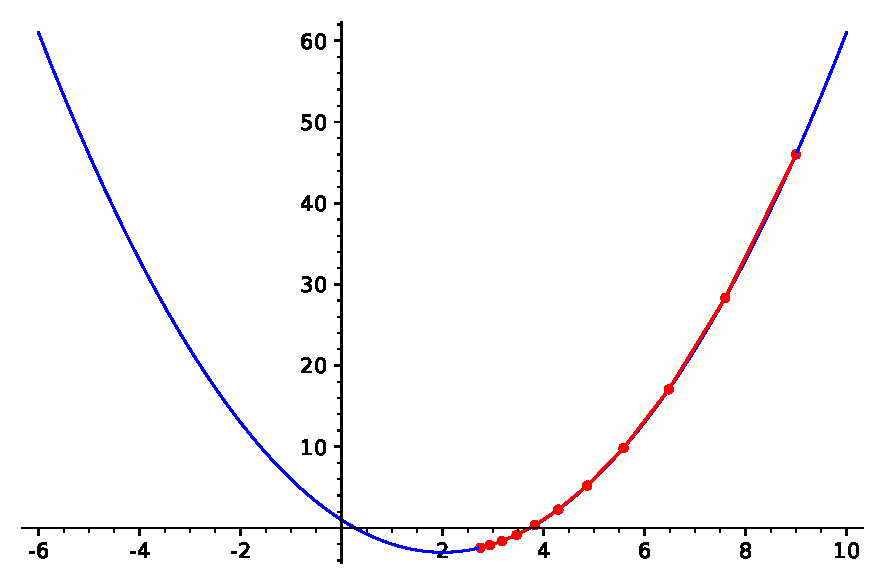
\includegraphics[scale=0.5]{imagenes/ejemplo1_1_maximodescensosimplificado.pdf}
	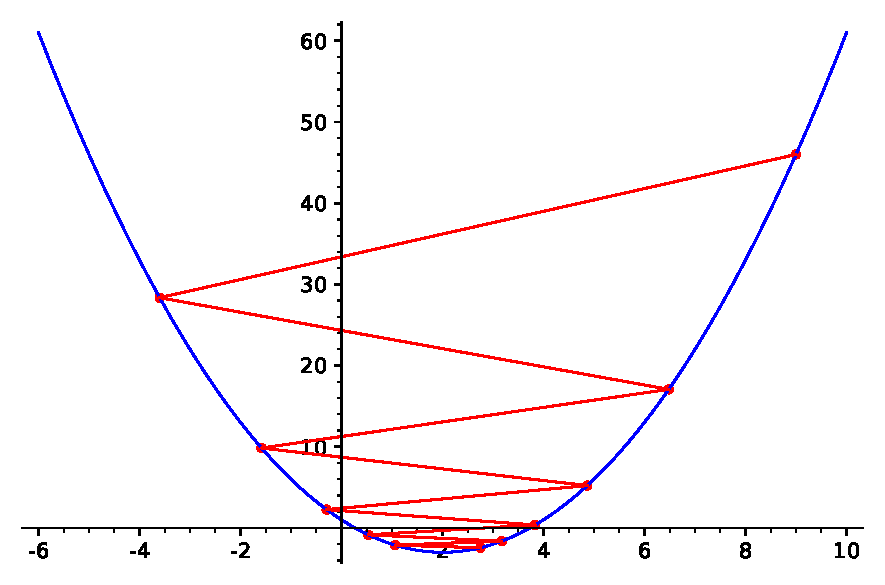
\includegraphics[scale=0.5]{imagenes/ejemplo1_2_maximodescensosimplificado.pdf}\\
	Ahora bien, si usamos el método aplicando backtracking, las iteraciones serán las siguiente: $$[9,3.4,2.28,2.056,2.0112,2.00224,2.00045,2.00009,2.00002,2.00001,2.00001]$$.\\
	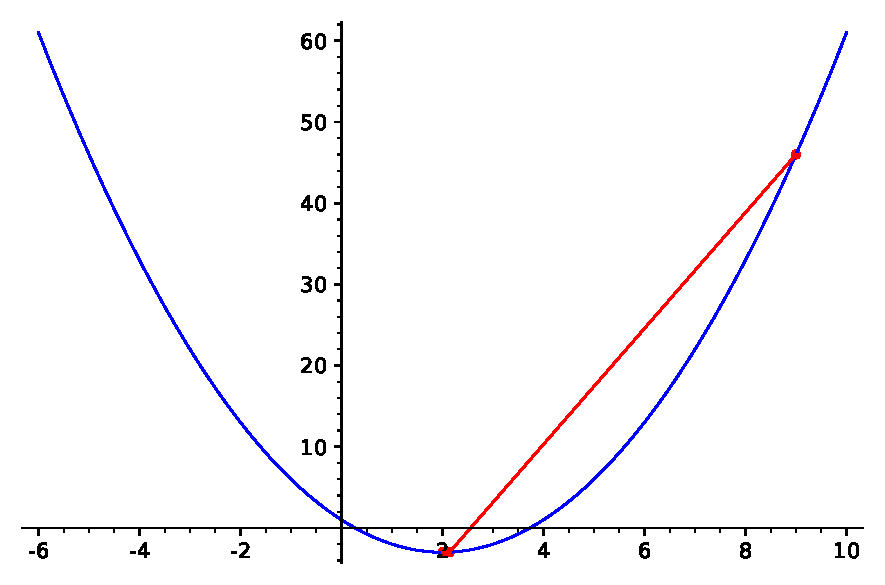
\includegraphics[scale=0.5]{imagenes/ejemplo1_maximodescenso.pdf}\centering \\
	Podemos observar que ahora es mucho más eficiente y no hace saltos innecesarios.
\end{example}
\begin{example}
	Tomamos ahora $g(x) = x^4 - 2x^3 + 2$ y el punto inicial $x_0 = 2$. Si tomamos un learning rate $L = 0.35$ obtendremos la siguiente gráfica:\\
	\begin{centering}
	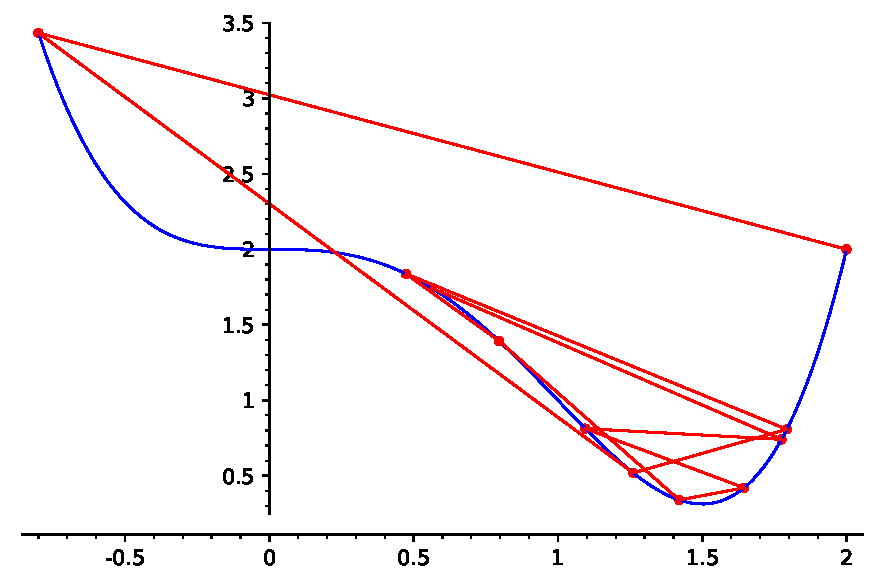
\includegraphics[scale=0.5]{imagenes/ejemplo2_maximodescensosimplificado.pdf} \\
	\end{centering}
	Es caótico e ineficiente. Pasa de largo la solución y nos nos ofrece un valor óptimo. Sin embargo, el algoritmo con backtracking nos da:\\
	\begin{centering}
	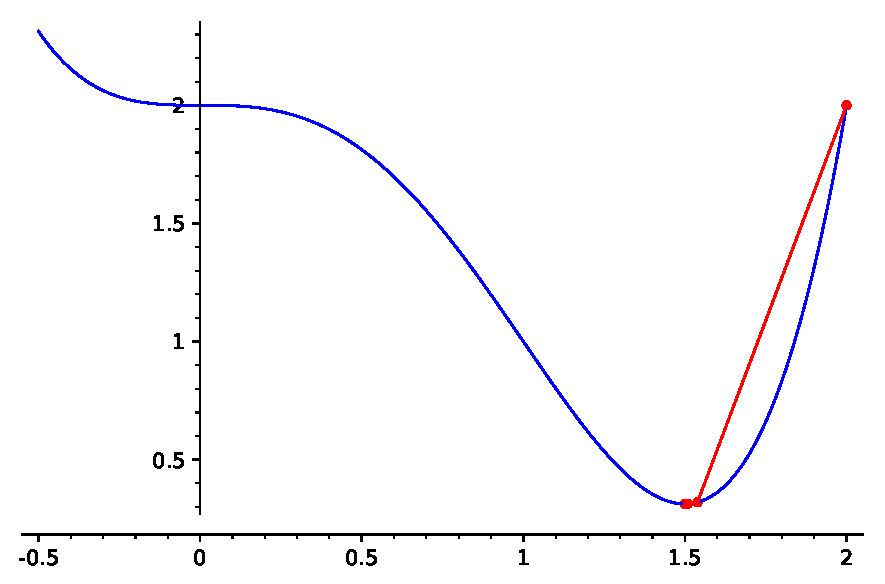
\includegraphics[scale=0.5]{imagenes/ejemplo2_maximodescenso.pdf} \\
	\end{centering}
	Donde las iteraciones han sido:
	\begin{equation*}
		\begin{aligned}
			[&2,1.7952,1.55165,1.51982,1.50809,1.50338,\\
			 &1.50142,1.50060,1.50026,1.50011,1.50005]
		\end{aligned}
	\end{equation*} 
\end{example}
\begin{example}
	Vamos a coger la función $f(x,y)=x^2+(y-2)^2$, y el punto inicial $(2,-2)$. Hacemos 10 iteraciones del método con backtracking y obtenemos:\\
	%\begin{centering}
		% width=15cm,height=5cm
	\begin{figure}[H]
		\centering
		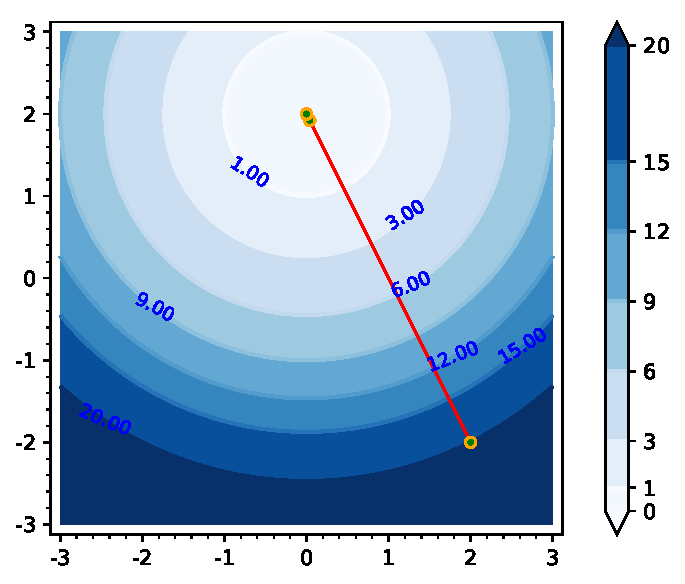
\includegraphics[scale = 0.6]{imagenes/ejemplo3_maximodescenso.pdf}
	\end{figure}
	%\end{centering}
	\begin{equation*}
		\begin{aligned}
			[&(2,-2),(0.40000,1.20000),(0.08000,1.84000),(0.01600,1.96800), \\
			(&0.00320,1.99360),(0.00064,1.99872),(0.00013,1.99974),(0.00003,1.99995),\\
			(&5.11999×10^{-6},1.99999),(1.02400×10^{-6},1.99999),
			(2.04799×10^{-7},1.99999)]
		\end{aligned}
	\end{equation*}
	
\end{example}

% Para reducir la complicación en términos de cálculos tomaremos $\alpha_1 < \alpha_2 < \alpha_3$ cercanos al valor buscado $h(\alpha)$:
%\begin{enumerate}
%	\item Cogemos $\alpha_1 = 0$ para reducir cálculos.
%	\item Encontramos un $\alpha_3$ con $h(\alpha_3 < h(\alpha_1))$.
%	\item Cogemos $\alpha_2 = \frac{\alpha_3}{2}$.
%\end{enumerate}
%Para aproximar la solución $p$ al problema de mínimos dado un x inicial:
%\[g(p) = \min_{x \in \mathbb{R}^n} g(x)\]
%Vamos a programar el siguiente algoritmo:
%
%\begin{algorithm}[H]
%	\floatname{algorithm}{Algoritmo}
%	\caption{Método de Broyden}
%	\textbf{Entrada: } \\
%	\hspace*{\algorithmicindent} $g$ \text{ - función real} \\
%	\hspace*{\algorithmicindent} $x_0$ \text{ - aproximación inicial} \\
%	\hspace*{\algorithmicindent} $TOL$ \text { - tolerancia} \\
%	\hspace*{\algorithmicindent} $N$ \text{ - número máximo de iteraciones} \\
%	\textbf{Salida:} \\
%	\hspace*{\algorithmicindent} $(x_1, \dots , x_k, g_1)$ \text{ - lista de aproximaciones al cero de } $g$
%	\begin{algorithmic}
%		\Procedure {}{}
%		%\State $x = x_0$
%		%\State $A = \Big(\frac{\partial f_i}{\partial x_j}\Big)_{1 \leq i , j \leq n}$ \Comment{Matriz Jacobiana de f}
%		%\State $x = x_1$ \Comment{Hallamos $x_1$ con el método de Newton}
%		\State $g_1 = g(x_1, \dots , x_N)$
%		\For{$k = 1,\dots,N$}
%			\If{$z_0 = 0$}
%				\State \Return $(x_1, \dots , xn, g_1)$ \Comment{Gradiente cero}
%			\Else
%				\State $z = \frac{z}{z_0}$ \Comment{Hacemos z un vector unitario}
%				\State $\alpha_1 = 0$
%				\State $\alpha_3 = 1$
%				\If{$g_3 \geq g_1$}
%					\State $\alpha_3 = \alpha_3 / 2$
%					\State $g_3 = g(x - \alpha_3 z)$
%					\If{$\alpha_3 < TOL/ 2$}
%						\State $\alpha_2 = \frac{\alpha_{3}}{2}$
%						\State \Return $(x_1, \dots , x_N , g_1)$ \Comment{Sin mejora posible}
%					\Else 
%						\State $g_2 = g(x- \alpha_2 z)$
%						\State $h_1 = \frac{g_2 - g_1}{\alpha_{2}}$
%						\State $ h_2 = \frac{g_3 - g_2}{\alpha_{3} - \alpha_{2}}$
%						\State $h_3 = \frac{h_2 - h_1}{\alpha_{3}}$ \Comment{La fórmula de diferencias divididas sirve para encontrar el cuadrático $P(\alpha) = g_1 + h_1 \alpha(\alpha-\alpha_{2})$, que interpola $h(\alpha)$ en $\alpha = 0$, $\alpha = \alpha_{2}$, $\alpha = \alpha_{3}$}
%						\State $\alpha_0 = 0.5(\alpha_{2} - \frac{h_1}{h_3})$ \Comment{El punto crítico de P ocurre en $\alpha_{0}$}
%						\State $g_0 = g(x - \alpha_{0}z)$
%						\State $g = g(x-\alpha z) = \min\{g_0, g_3\}$
%						\State $x = x - \alpha z$
%						\If{$|g - g_1| < TOL$}
%							\State \Return $(x_1, \dots , x_k , g)$ \Comment{El proceso tuvo éxito}
%						\Else
%							\State \Return \text{Excedido número máximo de iteraciones} \Comment{No hubo éxito}
%						\EndIf
%					\EndIf
%				\EndIf
%			\EndIf
%			\State $s = x_k - x_{k-1}$
%			\State $y = f(x_k) - f(x_{k-1})$
%			\State $x_{k+1} = x_k - A^{-1} f(x_k)$
%			\State $A = A + \frac{y_i + A s}{||s||_2^2} s^t$ 
%			\State \Return $x_k$ \Comment{El proceso tuvo éxito}
%		\EndFor
%		\EndProcedure
%	\end{algorithmic}
%\end{algorithm}

%\begin{itemize}
%\item INPUT número $n$ de variables; aproximación inicial $\mathbf{x}=\left(x_{1}, \ldots, x_{a}\right)^{y} ;$ tolerance $T O L ;$ número máximo de iteraciones $N .$
%\item OUTPUT $\quad$ solución aproximada $\mathbf{x}=\left(x_{1}, \ldots, x_{n}\right)^{\prime}$ ó un mensaje de fallo.
%\item Paso $1 \quad$ Sea $k=1$
%\item Paso $2 \quad$ Mientras $(k \leq N)$ hacer pasos $3-15$
%\item Paso $3 \quad$ Sea $g_{1}=g\left(x_{1}, \ldots, x_{n}\right) ; \quad\left(\right.$ Nota $\left.;\\ g_{1}=g\left(\mathbf{x}_{i}\right)-\right)$
%\item Paso 4 Si $z_{0}=0$ entonces OUTPUT ("gradiente cero");
%	$$
%	\text { OUTPUT }\left(x_{1}, \ldots, x_{n}, g_{1}\right)
%	$$
%	(Procedimiento completado, puede haber mínimo) STOP.\\
%	Paso $5 \quad$ Sea $z=z / z_{0}:$ (Hacer z vector unitario)
%	$$
%	\begin{array}{l}
%		\alpha_{1}=0 \\
%		\alpha_{3}=1 \\
%		g_{3}=g\left(\mathbf{x}-\alpha_{3} \mathbf{z}\right)
%	\end{array}
%	$$
%\item Paso 6 Mientras $\left(g 3 \geq g_{1}\right)$ hacer pasos 7 y 8.
%\item Paso $7 \quad$ Sea $a_{3}=\alpha_{3} / 2$
%	$$
%	z_{3}=g\left(\mathbf{x}-\alpha_{3} \mathbf{z}\right)
%	$$
%\item Paso $8 \quad$ Si $\alpha_{3}<T O L / 2$ entonces OUTPUT ('Sin mejora posible'): OUTPUT $\left(x_{1}, \ldots, x_{n}, g_{1}\right)$ (Procedimiento completado, puede haber mínimo.) STOP.
%\item Paso $9 \quad$ Sea $\alpha_{2}=\alpha_{3} / 2$
%	$$\\
%	g_{2}=g\left(\mathbf{x}-\alpha_{2} \mathbf{z}\right)
%	$$
%\item Paso $10 \quad$ Sea $h_{1}=\left(g_{2}-g_{1}\right) / \alpha_{2}$
%	$$
%	\begin{array}{l}
%		h_{2}=\left(g_{3}-g_{2}\right) /\left(\alpha_{3}-\alpha_{2}\right) \\
%		h_{3}=\left(h_{2}-h_{1}\right) / \alpha_{3}
%	\end{array}
%	$$
%	(Nota: La fórmula de Newton de diferencias divididas sirve para encontrar el cuadrático $P(\alpha)=g_{1}+h_{1} \alpha+h_{1} \alpha\left(\alpha-\alpha_{2}\right)$ que interpolan
%	$$
%	h(\alpha) \text { ar } \left.\alpha=0, \alpha=\alpha_{2}, \alpha=\alpha_{3} .\right)
%	$$
%\item Paso 11 Sea $\alpha_{0}=0.5\left(\alpha_{2}-h_{1} / h_{3}\right)$ : (El punto crítico de P ocurre en $\alpha_{0}$.)
%	$$
%	g_{0}=g\left(\mathbf{x}-\alpha_{0} \mathbf{z}\right)
%	$$
%\item Paso 12 . Encontrar $\alpha$ de $\left|\alpha_{0}, \alpha_{3}\right|$ tal que $g=g(\mathbf{x}-\alpha \mathbf{z})=\min \left\{g_{0}, g_{3}\right\}$ - 
%\item Paso $13 \quad$ Sea $\mathbf{x}=\mathbf{x}-\alpha \mathbf{z}$ \\
%\item Paso $14 \quad$ Si $\left|g-g_{1}\right|<T O L$ entonces OUTPUT $\left(x_{1}, \ldots, x_{m+}, g\right)$ 
%	(El proceso tuvo éxito.) STOP.
%\item Paso 15 Sea $k=k+1$ 
%\item Paso 16 OUTPUT ("Número máximo de iteraciones excedido"):
%	(El procedimiento no tuvo éxito.) STOP.
%\end{itemize}
%
%Existen otras técnicas como usar el polinomio multidimensional de Taylor para reemplazar la función $g$ de varias variables. En general todos los métodos de máximo descenso son linealmente convergentes independientemente de la aproximación inicial, pero en algunos casos convergen a algo que no es el mínimo absoluto de la función $g$.

\section{Método del gradiente conjugado}

El método del gradiente conjugado fue desarrollado por primera vez por los matemáticos Magnus R. Hestenes y Eduard Stiefel\cite{hestenes-stiefel-1952} como un método directo para resolver los sistemas de ecuaciones lineales de la forma $Ax=b$ donde $A$ es una matriz simétrica y definida positiva de dimensión $n\times n$ y $b$ es un vector de dimensión $n$. Este método es equivalente al de encontrar el mínimo de la forma cuadrática:
\begin{equation}\label{funcion-objectivo-cuadratico} f(x) = \frac{1}{2} x^t A x - b^t x \end{equation}
con $A$ simétrica y definida positiva, pues el mínimo de la función se da donde $x$ cumple que $f'(x)=Ax-b=0$.

Con algunas modificaciones, es posible extender el método para que funcione para cualquier función $f : \mathbb{R}^n \to \mathbb{R}$ para el que podamos estimar su matriz hessiana. Pero antes, para poder estudiar el método del gradiente conjugado no lineal, necesitaremos ver cómo funciona en el caso lineal.

\subsection{Gradiente conjugado lineal}
Comenzaremos considerando el problema de minimizar la función $f(x_k+ap_k)$ donde $x_k$ y $p_k$ son vectores constantes, $f$ es la función definida en \eqref{funcion-objectivo-cuadratico} y $a$ es un escalar. Por definición,

\[ f(x_k+ap_k) = \frac{1}{2} (x_k+ap_k)^t A (x_k+ap_k)-b^t(x_k+ap_k) \]

Diferenciando respecto $a$ obtenemos que:

\begin{align*} \frac{\partial f(x_k+ap_k)}{\partial a} &= p^tAx_k + ap_k^tAp_k -b^tp_k\\
	& = (x_k^tA-b^t)p_k +ap_k^tAp_k\\
	& = r_k^tp_k+ap_k^tAp_k
\end{align*}
donde hemos tomado $r_k = Ax_k-b$, al que denominaremos residuo.
Igualando la derivada a $0$, encontramos un mínimo para $f(x_k+ap_k)$ en $a_k$:
\[ a_k = -\frac{r_k^tp_k}{p_k^tAp_k}\]

De esta forma, dada una estimación $x_k$ y una dirección $p_k$, podemos encontrar el mínimo de $f$ restringida a la recta sobre $x_k$ paralela a $p_k$ tomando $x_{k+1} = x_k + ap_k$. Por otro lado, podemos calcular el nuevo residuo $r_{k+1}$ observando que:
\begin{align}
	r_{k+1} &= Ax_{k+1}-b\nonumber\\
	& = A(x_k+a_kp_k)-b\nonumber\\
	& =r_k+a_kAp_k\label{conj-cuad-resid}
\end{align}

En el método conjugado, elegimos en cada paso $k$ una dirección $p_k$ conjugada a todas las direcciones de los pasos anteriores (es decir, $p_k^tAp_j=0$ para todo $j<k$). Nos bastará con buscar una $\beta_k$ tal que la dirección $p_{k+1}=\beta_kp_k-r_{k+1}$ es conjugada con $p_k$. Entonces:

\[ 0=p_k^tAp_{k+1} = \beta_kp_k^tAp_k-p_k^tAr_{k+1}\]

Despejando $\beta_k$ tenemos:
\[ \beta_k = \frac{p_k^tAr_{k+1}}{p_kAp_k} \]

\subsection{Gradiente conjugado no lineal}

%Su funcionamiento como método directo es peor que el de la eliminación gaussiana, pues a pesar de que ambos requieren $n$ pasos para su resolución, los pasos que hay que realizar en el método del gradiente conjugado son más complejos que en el método de eliminación gaussiana, de ahí que posteriormente el matemático Reid planteara dicho método de forma iterativa. Esta es la forma que se utiliza en la actualidad y la principal ventaja es que puede resolver sistemas de ecuaciones lineales y no lineales de gran tamaño.
%
%Sea el sistema de ecuaciones lineales
%\begin{gather*}\left\{\begin{array}{c} a_{11}x_1+\ldots+a_{1n}x_n=b_1\\\vdots\\a_{n1}x_1+\ldots+a_{nn}x_n=b_n\end{array}\right.\end{gather*}
%que escrito de forma vectorial es $Ax=b$. Vamos a suponer que $A$ es una matriz invertible. Denotaremos a la matriz traspuesta de $A$ por $A^t$.
%
%Sean $x=(x_1, \ldots, x_n)$ e $y=(y_1, \ldots, y_n)$ dos vectores y $A=(a_{ij})_{i=1, \ldots, n}^{j=1, \ldots, n}\in\mathcal{M}_{n\times n}$ la matriz $A$ anterior.
%
%Si $a_{ij}=a_{ji}$, (i.e., $A=A^t$), diremos que $A$ es una \textbf{matriz simétrica}. Si esto ocurre, entonces diremos que $x$ e $y$ son dos \textbf{vectores conjugados o $A$-ortogonales} si verifican que
%\begin{gather*}\langle{x, Ay\rangle}=\langle{Ax, y\rangle}=0\end{gather*}
%es decir, dos vectores no nulos $x$ e $y$ son conjugados de $A$ si
%\begin{gather*}\langle{x, y\rangle}_A=0\end{gather*}
%
%\begin{definition} Dada la matriz \(A \in \mathcal{M}_{n\times n}\), decimos que es \textbf{definida positiva} si para todo vector $x$ no nulo se verifica
%\begin{gather*}\langle{x, Ax\rangle}>0\end{gather*}
%\end{definition}
%
%\begin{definition} Dada la matriz \(A \in \mathcal{M}_{n\times n}\), decimos que es \textbf{semidefinida positiva} si para todo vector $x\in V$ se verifica
%\begin{gather*}\langle{x, Ax\rangle}\geq0\end{gather*}
%\end{definition}
%La matriz $A$ y su traspuesta $A^t$ satisfacen la relación
%\begin{gather*}\langle{x, Ay\rangle}=\displaystyle\sum_{i, j=1}^na_{ij}x_iy_j=\langle{A^tx, y\rangle}\end{gather*}
%La expresión anterior es una extensión de la relación de ortogonalidad $\langle{x, y\rangle}=0$.
%
%
%\begin{definition} Sea $A$ una matriz de dimensión $n\times n$, $x$ y $b$ dos vectores de dimensión $n$ y $c$ un escalar. Denominaremos \textbf{forma cuadrática} a la función cuadrática escalar de un vector de la forma
%\begin{gather*}f(x)=\frac{1}{2}\langle{x, x\rangle}_A-\langle{b, x\rangle}+c\end{gather*}
%y definiremos su \textbf{gradiente} como
%\begin{gather*}f'(x)=\left[\frac{\partial f}{\partial x_1}, \frac{\partial f}{\partial x_2}, \ldots, \frac{\partial f}{\partial x_n}\right]^t\end{gather*}
%\end{definition}
%De lo anterior se deduce que
%\begin{gather*}f'(x)=\frac{1}{2}A^tx+\frac{1}{2}Ax-b\end{gather*}
%y si $A$ es una matriz simétrica, entonces nos queda que
%\begin{gather*}f'(x)=Ax-b\end{gather*}
%
%La solución del sistema $Ax=b$ la denotaremos $h$ de forma que $Ah=b$.La solución $h$ nos da un punto crítico de $f(x)$. Si además suponemos que la matriz $A$ es definida positiva, entonces $h$ será además el mínimo global de $f$.
%
%\begin{proof}
%	
%Suponemos $A$ simétrica y definida positiva. Sea $p \neq h$ vector. Tomemos $e = h - p$, entonces:
%
%\begin{align*}
%	f(p) = f(h+e) &= \frac{1}{2} (h+e)^TA(h+e)-b^T(h+e) + c = \\
%               	&= \frac{1}{2} h^TAh + h^TAe + \frac{1}{2} e^TAe -b^Th -b^Te  + c = \\
%               	&= f(h) + \frac{1}{2}e^TAe > f(h)
%\end{align*}
%
%\end{proof}
%
%Geométricamente, que $A$ es definida positiva nos asegura que no hay puntos de silla y que el mínimo es único. Lo cual será esencial para que el método del gradiente conjugado converja.
%
%Si $x$ es una estimación de $h$, la diferencia $r=b-Ax$ se denomina \textbf{residual} de $x$ como estimación de $h$.
%
%Normalmente, el vector residual se puede usar como una medida de bondad de la estimación $x_i$. Si no se encuentran errores de redondeo, podemos alcanzar una estimación $x_m<x_n$ la cual $r_m=0$. Esta será la solución buscada $h$.
%
%Para entender mejor el método del gradiente conjugado, conviene hablar antes del método del gradiente.
%
%En general, $x_{i+1}\in\mathbb{R}^n$ viene dado por \begin{gather*}x_{i+1}=x_i+a_ip_i\end{gather*}
%donde $a_i$ es el valor que refina la longitud del paso a lo largo de la dirección $p_i$. Lo ideal escoger como $p_i$ la dirección de máximo descenso a lo largo de la función $\phi$ en $x_i$ que viene dada por $-\nabla\phi(x_i)$. Escogiendo esta dirección, vemos que \begin{gather*}\nabla\phi(x_i)=Ax_i-b=-r_i\end{gather*}
%así que la dirección del gradiente de $\phi$ coincide con el residual.
%
%Para calcular el parámetro $a_i$ escribamos $\phi(x_{i+1})$ en función de un parámetro $a$:
%\begin{gather*}\phi(x_{i+1})=\frac{1}{2}\langle{x_i+ar_i, A(x_i+ar_i)\rangle}-\langle{x_i+ar_i, b\rangle}\end{gather*}
%Diferenciando respecto de $a$ e igualando a cero obtenemos que el valor de $a_i$ es
%\begin{gather*}a_i=\frac{\langle{r_i, r_i\rangle}}{\langle{r_i, Ar_i\rangle}}\end{gather*}
%que depende únicamente del residual en el paso $i$.
%
%Para calcular ahora el $r_{i+1}$, partiendo de la ecuación
%\begin{gather*}x_{i+1}=x_i+a_ir_i\end{gather*}
%obtenemos que
%\begin{gather*}r_{i+1}=r_i-a_iAr_i\end{gather*}
%
%En resumen, el método del gradiente consiste en, dado $x_0\in\mathbb{R}^n$ tomamos $r_0=b-Ax_0$ y desde $k=0, 1, \ldots$ hasta que el método converja hacemos el siguiente proceso iterativo 
%\begin{gather*}a_i=\frac{\langle{r_i, r_i\rangle}}{\langle{r_i, Ar_i\rangle}}\end{gather*}
%\begin{gather*}x_{i+1}=x_i+a_ir_i\end{gather*}
%\begin{gather*}r_{i+1}=r_i-a_iAr_i\end{gather*}
%
%Pasemos ahora a ver el método del gradiente conjugado.
%
%\underline{Paso inicial}. Escogemos una estimación $x_0$ de $h$ y calculamos el residual $r_0$ y la dirección $p_0$ mediante las fórmulas
%\begin{gather*}r_0=b-Ax_0  \\ p_0=r_0\end{gather*}
%
%La diferencia principal que distingue a ambos métodos reside en como se elige la dirección $p_i$. En general $p_i\neq r_i$. Por tanto, si calculamos de nuevo el parámetro $a_i$, diferenciando respecto de $a$, llegamos a que $\phi(x_{i+1})=\phi(x_i+ap_i)$ e igualando a cero, nos queda
%\begin{gather*}a_i=\frac{\langle{p_i, r_i\rangle}}{\langle{p_i, Ap_i\rangle}}\end{gather*}
%
%A partir de la ecuación
%\begin{gather*}x_{i+1}=x_i+a_ip_i\end{gather*}
%tenemos que
%\begin{gather*}r_{i+1}=r_i-a_iAp_i\end{gather*}
%y por medio del nuevo $a_i$ que tenemos, el nuevo residual $r_{i+1}$ se vuelve ortogonal a la dirección $p_i$, es decir, $\langle{p_i, r_{i+1}\rangle}=0$.
%
%La estrategia para la siguiente iteración es encontrar una nueva dirección $p_{i+1}$, de modo que $\langle{Ap_j, p_{i+1}\rangle}=0, j=0, \ldots, i$, esto es, las direcciones $p_j$ y $p_{i+1}$ son conjugadas. Primero vamos a probar que es posible encontrarlas:
%
%Supongamos que $p_0, p_1, \ldots, p_i$ $(i\geq1)$ son mutuamente conjugados, esto es, $\langle{Ap_j, p_k\rangle}=0$ para todo $j, k=0, \ldots, i, j\neq k$. Debe de cumplirse que $\langle{p_j, r_{i+1}\rangle}=0, j=0, \ldots, i$. Para demostrarlo, procedamos por el método de inducción sobre $i$:
%
%Para $i=0$, tenemos que
%\begin{gather*}r_1=r_0-a_0Ap_0\end{gather*}
%de este modo, como $\langle{Ap_j, p_k\rangle}$, nos queda que \begin{gather*}a_0=\frac{\langle{p_0, r_0\rangle}}{\langle{p_0, Ap_0\rangle}}.\end{gather*}
%Entonces
%\begin{gather*}\langle{p_0, r_1\rangle}=\langle{p_0, r_0\rangle}-\langle{p_0, r_0\rangle}=0.\end{gather*}
%
%Vamos a suponer que se cumple para $0, \ldots, i-1$ y veamos si se cumple para $i$.
%
%Tenemos que
%\begin{gather*}r_{i+1}=r_i-a_iAp_i\end{gather*}
%y por ser la matriz $A$ simétrica,
%\begin{gather*}\langle{p_j, r_{i+1}\rangle}=\langle{p_j, r_i\rangle}-a_i\langle{Ap_j, p_i\rangle}.\end{gather*}
%
%Para $j\neq i$, tenemos que $\langle{Ap_j, p_i\rangle}=0$ por ser conjugados, y además, por hipótesis de inducción, $\langle{p_j, r_i\rangle}=0$, luego $\langle{p_j, r_{i+1}\rangle}=0$.
%
%Para $j=i$, tenemos que $\langle{p_i, r_{i+1}\rangle}=0$ por la elección del $a_i$.
%
%Ya solo resta calcular la sucesión de direcciones $p_0, p_1, \ldots, p_i$ de modo que sean mutuamente conjugadas. Para ello, pongamos \begin{gather*}p_{i+1}=r_{i+1}-b_ip_i,\ i=0, 1, \ldots\end{gather*}
%donde inicialmente pondremos $p_0=r_0$ y donde $b_0, b_1, \ldots$ deben ser determinados. Utilizando la fórmula
%\begin{gather*}p_{i+1}=r_{i+1}-b_ip_i\end{gather*}
%en $\langle{Ap_i, p_{i+1}\rangle}=0$ obtenemos que
%\begin{gather*}b_i=\frac{\langle{Ap_i, r_{i+1}\rangle}}{\langle{Ap_i,p_i\rangle}}\ \ i=0, 1, \ldots\end{gather*}
%Pero usando la fórmula en $\langle{Ap_j, p_{i+1}\rangle}$ para $j\leq i-1$, obtenemos
%\begin{gather*}\langle{Ap_j, p_{i+1}\rangle}=\langle{Ap_j, r_{i+1}\rangle}-b_i\langle{Ap_j, p_i\rangle}\end{gather*}
%
%Tenemos que probar que
%\begin{gather*}\langle{Ap_j, p_{i+1}\rangle}=\langle{Ap_j, r_{i+1}\rangle}-b_i\langle{Ap_j, p_i\rangle}=0,\ j\leq i-1.\end{gather*}
%Pues bien, por hipótesis de inducción sobre $j\leq i-1$ tenemos que $\langle{Ap_j, p_i\rangle}=0$. Veamos ahora que $\langle{Ap_j, r_{i+1}\rangle}=0$.
%
%Sea $v_i=\langle{p_0, \ldots, p_i\rangle}$. Si cogemos $p_0=r_0$ teniendo en cuenta que
%\begin{gather*}p_{i+1}=r_{i+1}-b_ip_i\end{gather*}
%vemos que el $v_i$ se puede representar como $v_i=\langle{r_0, \ldots, r_i\rangle}$. Por tanto, $Ap_i\in v_{i+1}$ debido a que \begin{gather*}r_{i+1}=r_i-a_iAp_i.\end{gather*}
%
%Ahora como $r_{i+1}$ es ortogonal a todo vector de $v_i$, nos queda entonces que
%\begin{gather*}\langle{Ap_j, r_{i+1}\rangle}=0,\ j=0, \ldots, i-1.\end{gather*}
%
%En resumen, tras coger las nuevas direcciones como
%\begin{gather*}p_{i+1}=r_{i+1}-b_ip_i\end{gather*}
%y el parámetro $a$ como
%\begin{gather*}a_i=\frac{\langle{p_i, r_i\rangle}}{\langle{p_i, Ap_i\rangle}}\end{gather*}
%obtenemos el método del gradiente conjugado.
%
%En total, dado $x_0\in\mathbb{R}^n$ tomemos como residuo inicial $r_0$ y dirección inicial $p_0$, respectivamente
%\begin{gather*}r_0=b-Ax_0 \\ p_0=r_0.\end{gather*}
%Entonces para $i=0, 1, \ldots$ hasta que converja, hacemos
%\begin{gather*}a_i=\frac{\langle{p_i, r_i\rangle}}{\langle{p_i, Ap_i\rangle}}\end{gather*}
%\begin{gather*}x_{i+1}=x_i+a_ip_i\end{gather*}
%\begin{gather*}r_{i+1}=r_i-a_iAp_i\end{gather*}
%\begin{gather*}b_i=\frac{\langle{r_{i+1}, Ap_i\rangle}}{\langle{p_i, Ap_i\rangle}}\end{gather*}
%\begin{gather*}p_{i+1}=r_{i+1}-b_ip_i\end{gather*}
%
%
%Los residuales $r_0, r_1, \ldots$ son mutuamente ortogonales y los vectores de dirección $p_0, p_1, \ldots$ son mutuamente conjugados, es decir, $\langle{r_i, r_j\rangle}=0$ son ortogonales y $\langle{p_i, Ap_j\rangle}=0$ son $A$-ortogonales para todo $i\neq j$.
%%
%Para implementar el método del gradiente conjugado de forma no lineal, no podremos usar la fórmula recursiva para el residuo, pues el algoritmo va ganando demasiada complejidad, y la elección de $b_i$ son significativamente distintas.

En el caso no lineal, nuestro problema de optimización será

\begin{equation}\label{min-f}
	\min_{x \in \mathbb{R}^n} f(x)
\end{equation}
donde $f : \mathbb{R}^n \to \mathbb{R}$ y su gradiente $f'$ es continuo.

Hay varios métodos de generalizar el método del gradiente conjugado para el caso de una función $f$ no lineal. Los que vamos a considerar siguen la estructura:

\begin{enumerate}
	\item En $k=0$, tomar una estimación $x_k$, una dirección de descenso inicial $p_k=-f'(x_k)$ y un residuo inicial $r_k=p_k$.
	\item Calcular un $a_k$ que minimiza $f(x_k+a_k p_k)$.
	\item Actualizar la estimación $x_{k+1} = x_k + a_k p_k$.
	\item Tomar $r_{k+1}=-f'(x_{k+1})$. Si $\|r_{k+1}\|$ es pequeño, parar.
	\item Calcular un $\beta_{k+1}$
	\item Actualizar la dirección de búsqueda $p_{k+1} = \beta_{k+1} p_k-f'(x_{k+1})$
	\item Repetir desde el paso 2 incrementando $k$ en 1.
\end{enumerate}

La diferencia esencial con el caso lineal es que los pasos 2 y 5 no se pueden realizar con tanta facilidad. Para el paso 2, podemos recurrir a uno de varios métodos de búsqueda lineal. En particular, el problema se puede transformar a la búsqueda de ceros de la expresión $[f'(x_k + a_k p_k)]^{t} p_k$. Para calcular el paso 5, en el caso lineal calculamos una $\beta_k$ tal que la $p_{k+1}$ del paso 6 fuera conjugada con $p_k$, pero en el caso no lineal varios autores han propuesto varias elecciones de $\beta_k$. Vamos a ver la elección de Fletcher-Reeves (FR) y de Polak-Rivière (PR):

\[\beta_{k+1}^{FR} = \frac{r^t_{k+1} r_{k+1}}{r^t_k r_k} = \frac{\|r_{k+1}\|^2}{\|r_k\|^2} = \frac{\|f'(x_{k+1})\|^2}{\|f'(x_k)\|^2} \]
\[\beta_{k+1}^{PR} = \frac{r^t_{k+1} (r_{k+1}-r_k)}{r^t_k r_k} \]

\subsection{Convergencia de los métodos del gradiente conjugado}

Seguiremos la notación de la sección anterior, pero impondremos las siguientes condiciones adicionales a la función $f$ y la estimación inicial $x_0$:
\begin{itemize}
	\item El conjunto $\mathcal{L}=\{x : f(x) \leq f(x_0)\}$ está acotado.
	\item En un entorno de $\mathcal{L}$, el gradiente $f$' es función lipschitziana.
\end{itemize}

La convergencia del método del gradiente conjugado no lineal dependerá de nuestra elección de cómo obtener $a_k$ y $\beta_k$. Para el cálculo de $a_k$ --la búsqueda en línea-- se puede recurrir a métodos exactos como el de máximo descenso, pero en la práctica la convergencia es lenta. En su lugar, nos resignaremos a buscar $a_k$ que en lugar de minimizar $f(x_k+a_kp_k)$, cumpla las condiciones para garantizar la convergencia del método del gradiente conjugado.

Como ya vimos en el apartado anterior, una forma de acotar la dirección de búsqueda en línea era mediante la condición de Armijo \ref{armijo}. Sin embargo, en el problema que nos atañe ahora puede ocurrir que el paso sea tan pequeño que $x_k$ no converja a un minimizador local. Entonces, necesitamos otra condición que acote inferiormente, la cual denominaremos "condición de curvatura".

\begin{definition}
	Dado el problema de optimización \ref{min-f} y una dirección de descenso $p_k$, diremos que $a_k$ cumple las \textbf{condiciones de Wolfe} si:
	\begin{itemize}
		\item $f(x_k+a_kp_k) \leq f(x_k) + \sigma_1 a_k f'(x_k)^t p_k$
		\item $f'(x_k+a_kp_k)^t p_k \geq \sigma_2 f'(x_k)^t p_k$
	\end{itemize}
	donde $0 < \sigma_1 < \sigma_2 < 1$. Si además cumple que
	\begin{itemize}
		\item $|f'(x_k+a_kp_k)^t p_k| \leq -\sigma_2 f'(x_k)^t p_k$
	\end{itemize}
	diremos que cumple las \textbf{condiciones fuertes de Wolfe}
\end{definition}

Dado un método de gradiente conjugado, tomemos $\theta_k$ como el ángulo entre $-f'(x_k)=r_k$ y $p_k$. Tenemos que $\cos (\theta_k) = -f'(x_k)^tp_k / (\|f'(x_k)\|\|p_k\|)$.
\begin{definition}
	Diremos que el método de gradiente conjugado cumple la \textbf{condición de Zoutendijk} si:
	\[
		\sum_{k=1}^\infty \cos^2 (\theta_k) \|f'(x_k)\|^2 < \infty
	\]
\end{definition}

Con estas condiciones, ya podemos estudiar la convergencia de los métodos del gradiente conjugado siempre y cuando $|\beta_k|$ esté acotado por $\beta_k^{FR}$. Lo primero que veremos es que las condiciones de Wolfe implican la condición de Zoutendijk en ciertos casos.

\begin{theorem}
	Dado un método de gradiente conjugado para minimizar $f$ tal que $a_k$ cumple las condiciones de Wolfe, entonces el método cumple la condición de Zoutendijk.
	
\begin{proof}
	Restando $f'(x_k)^tp_k$ a los dos lados de la segunda condición de Wolfe obtenemos:
	\[ (f'(x_k+a_kp_k) - f'(x_k))^tp_k \geq (\sigma_2 - 1)f'(x_k)p_k \]
	Por otro lado, como estamos suponiendo que $f'$ es lipschitziana de constante de Lipschitz $L$:
	\[ |f'(x_k+a_kp_k) - f'(x_k))^tp_k| \leq L \|x_k+a_kp_k-x_k\| \|p_k\| = L a_k \|p_k\|^2 \]
	De las dos inecuaciones se deduce entonces que:
	\[ a_k \geq \frac{\sigma_2-1}{L\|p_k\|^2} f'(x_k)^tp_k\]
	Multipliquemos los dos lados de la inecuación por $-1$ y apliquémoslo sobre la primera condición de Wolfe:
	\[ f(x_k+a_kp_k) \leq f(x_k) - \sigma_1 \frac{\sigma_2-1}{L\|p_k\|^2} (f'(x_k)^tp_k)^2\]
	Tomando $A=\sigma_1(1-\sigma_2)/L$ y usando la definición de $\theta_k$:
	\[ f(x_{k+1}) \leq f(x_k) - A\cos(\theta_k)^2\|f'(x_k)\|^2 \]
	Aplicando reiteradamente esta desigualdad podemos llegar a que:
	\[ f(x_{k+1}) \leq f(x_0) - A\sum_{j=0}^k \cos^2(\theta_j) \|f'(x_j)\|^2 \]
	Ahora bien, como estábamos suponiendo que que $\mathcal{L}=\{x : f(x)\leq f(x_0)\}$ está acotado, podemos deducir que $f(x_{k+1})-f(x_0)$ está acotado por una constante para cualquier $k$, luego
	\[ \sum_{k=0}^\infty \cos^2(\theta_k)\|f'(x_k)\|^2 < \infty\]
\end{proof}
\end{theorem}
Obsérvese que la condición de Zoutendijk implica en particular que $\cos(\theta_k)\|f'(x_k)\|^2\to 0$, por lo tanto, si $\cos(\theta_k)\geq \delta>0$ para todo $k$, podemos asegurar que $\|f'(x_k)\|\to 0$.

\begin{lemma}
	Consideremos un método del gradiente conjugado donde $\alpha_k$ satisface las condiciones fuertes de Wolfe con $\sigma_2<\frac{1}{2}$ y $|\beta_k| \leq \beta_k^{FR}$ para todo $k$, entonces:
	\[
		-1- \frac{\sigma_2}{1-\sigma_2} \leq \frac{f'(x_k)^t p_k}{\|f'(x_k)\|^2} \leq -1+\frac{\sigma_2}{1-\sigma_2}, \quad \forall k\geq 0
	\]
\begin{proof}
	Lo demostraremos por inducción. El resultado es cierto para $k=0$, pues como $p_0=-f'(0)$, basta que se cumpla que:
	\[ -1- \frac{\sigma_2}{1-\sigma_2} \leq -1 \leq -1+\frac{\sigma_2}{1-\sigma_2} \]
	que es cierto cuando $0<\sigma_2<1$. Tomaremos como hipótesis de inducción que el lema es cierto para $k$ y lo demostraremos para $k+1$. Del paso 6 del método conjugado, tenemos que:
	\begin{align}
		\frac{f'(x_{k+1})^t p_{k+1}}{\|f'(x_{k+1})\|^2} &= \frac{f'(x_{k+1})^t (\beta_{k+1}p_k - f'(x_{k+1}))}{\|f'(x_{k+1})\|^2}\nonumber\\
		&= \frac{f'(x_{k+1})^t \beta_{k+1}p_k}{\|f'(x_{k+1})\|^2}-1\nonumber\\
		&= \frac{\beta_{k+1}f'(x_{k+1})^tp_k}{\beta_{k+1}^{FR} \|f'(x_k)\|^2} - 1\label{wolfe-convergence-proof-eq1}
	\end{align}
	Por las condiciones fuertes de Wolfe sabemos que
	\[ \sigma_2 |\beta_{k+1}|f'(x_k)^tp_k\leq \beta_{k+1} f'(x_{k+1})^t p_k \leq - \sigma_2 |\beta_{k+1}|f'(x_k)^tp_k\]
	Entonces, usando \eqref{wolfe-convergence-proof-eq1} tenemos que:
	\[ -1+\sigma_2 \frac{|\beta_{k+1}|f'(x_k)^tp_k}{\beta_{k+1}^{FR}\|f'(x_k)\|^2}\leq \frac{f'(x_{k+1})^t p_{k+1}}{\|f'(x_{k+1})\|^2} \leq -1 - \sigma_2 \frac{|\beta_{k+1}|f'(x_k)^tp_k}{\beta_{k+1}^{FR}\|f'(x_k)\|^2}\]
	Aplicando la hipótesis de inducción:
	\[ -1- \frac{|\beta_{k+1}|}{\beta_{k+1}^{FR}} \frac{\sigma_2}{1-\sigma_2} \leq \frac{f'(x_{k+1})^t p_{k+1}}{\|f'(x_{k+1})\|^2} \leq -1+ \frac{|\beta_{k+1}|}{\beta_{k+1}^{FR}} \frac{\sigma_2}{1-\sigma_2}\]
	Como $|\beta_{k+1}|\leq \beta_{k+1}^{FR}$ y debido a que $0<\sigma_2<1$ tenemos que $0<\sigma_2/(1-\sigma_2)<1$, se deduce que:
	\[
	-1- \frac{\sigma_2}{1-\sigma_2} \leq \frac{f'(x_{k+1})^t p_{k+1}}{\|f'(x_{k+1})\|^2} \leq -1+\frac{\sigma_2}{1-\sigma_2}
	\]
	Con esto queda concluida la demostración por inducción.
\end{proof}
\end{lemma}
Este lema nos demuestra que la dirección $p_k$ es realmente una dirección de descenso respecto a $f'(x_k)$ en cada iteración $k$. Además multiplicando por $-\|f'(x_k)\|/\|p_k\|^2$ nos da el siguiente corolario.
\begin{corollary}\label{zoutedijk-corol}
	\[
	\left(1-\frac{\sigma_2}{1-\sigma_2}\right)\frac{\|f'(x_k)\|}{\|p_k\|} \leq \cos(\theta_k) \leq \left(1+\frac{\sigma_2}{1-\sigma_2}\right)\frac{\|f'(x_k)\|}{\|p_k\|}
	\]
\end{corollary}

\begin{theorem}\label{teorema-convergencia-wolfe}
	Consideremos un método del gradiente conjugado donde $\alpha_k$ satisface las condiciones fuertes de Wolfe con $\sigma_2<\frac{1}{2}$ y $|\beta_k| \leq \beta_k^{FR}$ para todo $k$, entonces para el método converge.
	
\begin{proof}
	Que el método converja quiere decir que el residuo se hace tan pequeño como queramos. Es decir, dado cualquier $\epsilon > 0$, existe $K>0$ tal que $\|r_K\|<\epsilon$.
	
	Del paso 6 del método del gradiente conjugado resulta que:
	\[ \|p_{k+1}\|^2 \leq \beta_{k+1}^2\|p_k\|^2 + \|f'(x_{k+1})\|^2+2|\beta_{k+1}|f'(x_{k+1})^tp_k \]
	Obsérvese además que el lema anterior implica que:
	\[ |f'(x_{k+1})^tp_k| \leq -\sigma_2f'(x_k)^tp_k\leq \frac{\sigma_2}{1-\sigma_2}\|f'(x_k)\|^2 \]
	Por lo tanto:
	\begin{align*}
		\|p_{k+1}\|^2 & \leq \beta_{k+1}^2\|p_k\|^2 + \|f'(x_{k+1})\|^2+2\frac{\sigma_2}{1-\sigma_2}|\beta_{k+1}|\|f'(x_k)\|^2\\
		& = \beta_{k+1}^2\|p_k\|^2 + \|f'(x_{k+1})\|^2+2\frac{\sigma_2}{1-\sigma_2}\frac{|\beta_{k+1}|}{\beta_{k+1}^{FR}}\|f'(x_{k+1})\|^2\\
		& \leq \beta_{k+1}^2\|p_k\|^2 + \frac{1+\sigma_2}{1-\sigma_2}\|f'(x_{k+1})\|^2
	\end{align*}
	
	Tomando $\hat{\sigma}=(1+\sigma_2)/(1-\sigma_2)$ y repitiendo esta desigualdad reiteradamente usando que $\beta_k^2\leq(\beta_k^{FR})^2$:
	\begin{align*}
		\|p_{k+1}\|^2 & \leq \hat{\sigma}\|f'(x_{k+1})\|^2+ (\beta_{k+1}^{FR})^2\|p_k\|^2 \\
		& \leq \hat{\sigma}\|f'(x_{k+1})\|^2+ (\beta_{k+1}^{FR})^2\left( \hat{\sigma}\|f'(x_k)\|^2+(\beta_{k+1}^{FR})^2\|p_{k-1}\|^2\right)\\
		& \dots\\
		& \leq \hat{\sigma}\|f'(x_{k+1})\|^2+ (\beta_{k+1}^{FR})^2\left( \hat{\sigma}\|f'(x_k)\|^2+(\beta_{k+1}^{FR})^2\|p_{k-1}\|^2+(\dots+(\beta_1^{FR})^2\|p_0\|^2)\dots\right)\\
		& = \hat{\sigma} \|f'(x_k)\|^4 \sum_{j=0}^k \|f'(x_j)\|^{-2}
	\end{align*}
	Ahora bien, como $f'$ es continua, está acotada superiormente en el conjunto compacto $\mathcal{L}$ por un $\gamma$, tenemos que:
	\begin{equation} \label{conj-conv-cota-direccion} \|p_{k+1}\|^2 \leq \hat{\sigma}\gamma^4 \sum_{j=0}^k \|f'(x_j)\|^{-2}
\end{equation}
	
	Supongamos ahora que el método no converge, por lo que existe un $C>0$ tal que para todo $k$ se tiene que $\|r_k\|\geq C$. Por lo tanto, $\|f'(x_k)\|^2\geq C^2$. Usando esto en la desigualdad \eqref{conj-conv-cota-direccion} tenemos que:
	\begin{equation}
		\|p_{k+1}\|^2 \leq \hat{\sigma}\frac{\gamma^4}{C^2} (k+1)
	\end{equation}
	Por lo tanto la serie $\sum_{k=0}^\infty \dfrac{1}{\|p_{k+1}\|^2}$ diverge. En consecuencia, también diverge la siguiente serie:
	\[ \left(1-\frac{\sigma_2}{1-\sigma_2}\right)^2 \sum_{k=0}^\infty \dfrac{C^4}{\|p_{k+1}\|^2} \]
	Sin embargo:
	\begin{align*}
		\left(1-\frac{\sigma_2}{1-\sigma_2}\right)^2 \sum_{k=0}^\infty \dfrac{C^4}{\|p_{k+1}\|^2} & \leq \left(1-\frac{\sigma_2}{1-\sigma_2}\right)^2 \sum_{k=0}^\infty \dfrac{\|f'(x_k)\|^4}{\|p_{k+1}\|^2}\\
		& \leq \sum_{k=0}^\infty \cos^2(\theta_k) \|f'(x_k)\|^2
	\end{align*}
	Aquí hemos usado el corolario \ref{zoutedijk-corol}. Llegamos a una contradicción, pues sabemos que esta serie converge, luego no puede acotar por encima una serie positiva que diverge. Llegamos entonces a la conclusión de que el método converge por reducción al absurdo.
\end{proof}
\end{theorem}

De esta forma hemos visto que FR converge bajo ciertas condiciones de regularidad del conjunto $\mathcal{L}=\{x : f(x) \leq f(x_0)\}$, que en la práctica se dan cuando $x_0$ está suficientemente cerca del mínimo.

En el caso del método PR, no siempre se da la convergencia y es posible encontrar funciones de manera que el método quede atrapado en un bucle infinitamente. Sin embargo, podemos realizar correcciones de $\beta^{PR}$ para que sí converja. Una posibilidad es acotar la $\beta^{PR}$ por $\beta^{FR}$, que denominaremos $\beta_k^{PRFR}$:
\[ \beta_k^{PRFR} = \begin{cases}
	\beta_k^{FR} & \text{si }|\beta_k^{PR}|>\beta_k^{FR} \\
	\beta_k^{PR} & \text{si }|\beta_k^{FR}|\leq\beta_k^{FR}
\end{cases}\]
De esta manera, podríamos aplicar el teorema \ref{teorema-convergencia-wolfe} para garantizar la convergencia. Otra opción es usar un reinicio de dirección de descenso, que significa imponer $\beta_{k+1}=0$ para que la nueva dirección de búsqueda sea $p_{k+1} = \beta_{k+1} p_k - f'(x_{k+1}) = -f'(x_{k+1})$. De esta forma, es equivalente a reiniciar el método tomando de estimación inicial $\hat{x}_0$ la última estimación antes de reiniciar $x_{k+1}$. Para evitar los bucles infinitos del método de PR, basta con reiniciar cuando $\beta_k<0$:
\[ \beta_k^{PR+} = \max\{\beta_k^{PR}, 0\} \]

En el análisis anterior sobre la convergencia de FR podemos explicar las limitaciones de FR según el comportamiento del gradiente. Supongamos que en la bucle $k$, obtenemos que $\cos(\theta_k)\approx 0$, es decir que $p_k$ es casi ortogonal a $f'(x_k)$. En ese caso lo más probable es que la búsqueda lineal no mejore significativamente la estimación y $x_{k+1}\approx x_k$. Entonces $\|f'(x_{k+1})\|\approx\|f'(x_k)\|$ luego $\beta_{k+1}^{FR} \approx 1$. Además, por el corolario \ref{zoutedijk-corol} tenemos que $\|p_k\|\gg \|f'(x_k)\|$, luego $p_{k+1} \approx p_k$. En consecuencia, $p_{k+1}$ también será casi ortogonal a $f'(x_{k+1})$ y la situación se extenderá durante más iteraciones provocando que el método converja más lentamente. Por otro lado, en el caso del método PR, tenemos que si $f'(x_k) \approx f'(x_{k+1})$, entonces $r_{k+1} \ \approx r_k$, luego $\beta_{k+1}^{PR} \approx 0$. En consecuencia, la nueva dirección de búsqueda será aproximadamente la dirección de máximo descenso. Por esto, PR suele acabar en menos iteraciones que FR en la práctica.

%El método de PR es, generalmente, mucho más eficiente, pero en ocasiones puede quedarse atrapado en un bucle infinito. Sin embargo, si hacemos una correcta elección de $b = \max\{b^{PR},0\}$, podemos garantizar la convergencia.

%En resumen, el método será el siguiente:

%\[p_0 = r_ 0 = - f'(x_0)\]
%\[a_{i+1} = \min\{f(x_i + a_i p_i)\}\]
%\[x_{i+1} = x_i + a_i p_i\]
%\[r_{i+1} = -f(x_{i+1}) \]
%\[b_{i+1} = b_{i+1}^{FR} \; \text{ó} \; \max\{b^{PR},0\}\]
%\[p_{i+1} = r_{i+1} - b_{i+1}p_i\]

%Si $f$ es una función polinómica, podemos usar un algoritmo eficiente para encontrar sus ceros. Por ejemplo, el método de Newton-Raphson o el método de la secante. Ambos requieren que $f \in \mathcal{C}^2$. Además,  Newton-Raphson requiere que se pueda calcular la segunda derivada de $\frac{\partial f(x + a p)}{\partial a}$. Para ello, aproximamos por el método de Taylor:

%\[f(x + a p)  \approx f(x) + a \Big[ \frac{\partial}{\partial a} f(x + a p) \Big]_{a=0} + \frac{a^2}{2} \Big[ \frac{\partial^2}{\partial a^2} f(x + a p) \Big]_{a=0} =\]
%\[ = f(x) + a[f'(x)]^T\ p + \frac{a^2}{2} p^T f''(x) p \]
%\[ \frac{\partial}{\partial a} f(x + a p) =  [f'(x)]^T\ p + a p^T f''(x) p \]

%Donde $f''(x)$ es la matriz Hessiana.

Vamos a ilustrar el método con un ejemplo:

\begin{example}
	Consideremos el problema de minimizar la función
	\[ f(x,y) = x^4 - 2x^2y+x^2+y^2-2x+1 \]
	Con la estimación inicial $(-2, -2)$. Su gradiente es:
	\[ f'(x,y) = \begin{pmatrix}
		4x^3-4xy+2x-2\\
		2x^2+2y
	\end{pmatrix}\]

Resolvemos programáticamente el problema usando Sage. Para la búsqueda lineal, usamos un implementación proporcionada por la librería scipy. Para el cálculo de $\beta$, usamos tanto FR como PR para comparar. Vemos que FR tarda 21 iteraciones en acabar, mientras PR sólo tarda 8. Véase la siguiente figura y tabla para más detalle.

\begin{figure}[h]
	\centering
	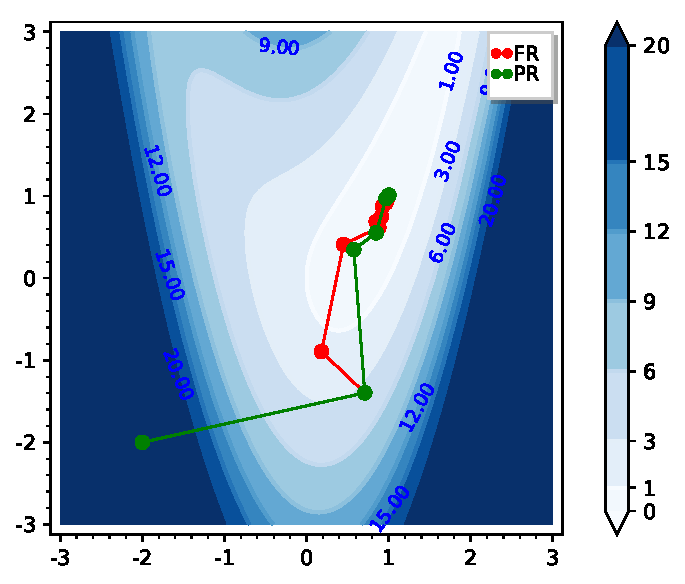
\includegraphics{imagenes/ejemplo_gradConjugado.pdf}
	\caption{Estimaciones tomadas por métodos de gradiente conjugado FR y PR}
\end{figure}

\begin{table}
\small
\begin{tabular}{llllll}
	Estimaciones FR & $\beta^{FR}$ & Error FR & Estimaciones PR & $\beta^{PR}$ & Error PR \\ \hline
	-2.0, -2.0 &  & $55.317267$ & -2.0, -2.0 &  & $55.317267$ \\
	0.710091, -1.397758 & $0.012329$ & $6.142219$ & 0.710091, -1.397758 & $0.082515$ & $6.142219$ \\
	0.182202, -0.89588 & $0.11587$ & $2.090795$ & 0.576622, 0.347088 & $0.136054$ & $0.880906$ \\
	0.451325, 0.411295 & $0.535195$ & $1.529563$ & 0.848701, 0.551205 & $0.56298$ & $0.433627$ \\
	0.87987, 0.615812 & $0.08585$ & $0.448165$ & 0.967816, 0.969583 & $0.613928$ & $0.202778$ \\
	0.84808, 0.688793 & $0.218726$ & $0.209598$ & 1.003708, 1.01064 & $-0.034055$ & $0.008432$ \\
	0.911726, 0.745441 & $1.093652$ & $0.219193$ & 1.001219, 1.001683 & $1.010095$ & $0.005675$ \\
	0.928343, 0.874529 & $0.768798$ & $0.192191$ & 0.999897, 0.999547 & $-0.128815$ & $0.00092$ \\
	0.967755, 0.914951 & $0.060409$ & $0.047237$ &  &  &  \\
	0.966196, 0.930742 & $1.460643$ & $0.05709$ &  &  &  \\
	0.998662, 0.990128 & $0.272188$ & $0.029785$ &  &  &  \\
	0.997323, 0.994147 & $0.013676$ & $0.003483$ &  &  &  \\
	0.997907, 0.994432 & $0.782209$ & $0.003081$ &  &  &  \\
	0.999031, 0.998409 & $1.210753$ & $0.00339$ &  &  &  \\
	0.999631, 0.998938 & $0.064392$ & $0.00086$ &  &  &  \\
	0.999586, 0.999097 & $0.406375$ & $0.000548$ &  &  &  \\
	0.999813, 0.999378 & $2.064417$ & $0.000788$ &  &  &  \\
	0.999879, 0.999787 & $0.212099$ & $0.000363$ &  &  &  \\
	0.999937, 0.999826 & $0.099217$ & $0.000114$ &  &  &  \\
	0.999931, 0.999854 & $0.794073$ & $0.000102$ &  &  &  \\
	0.999978, 0.999919 & $1.562019$ & $0.000127$ &  &  &  \\
\end{tabular}
\end{table}
\end{example}

\chapter{Método de continuación homotópica}

Los métodos de homotopía o continuación introducen un problema de la forma $F(x) = 0$, cuya solución estamos buscando, donde $F: \mathbb{R}^n \longrightarrow \mathbb{R}^n$, que asumiremos como suave, también entendido como clase $\mathcal{C}^\infty$.
Para este tipo de problema, asumimos que tenemos información escasa a priori de la solución. Si por el contrario tenemos cierta idea sobre el cero que buscamos, podríamos calcularlo mediante un algoritmo como el de Newton o similar.
Como remedio a esta gran falta de información previa es que definiremos una homotopía o deformación que nos ayudará a elegir el punto inicial.

El método consiste en considerar una homotopía $H$ parametrizada por $\lambda$ tal que $H(x,1)=F(x)$ y $H(x,0)=G(x)$ para alguna función $G:\mathbb{R}\to\mathbb{R}^n$ de la que podamos obtener sus ceros fácilmente.
Con cierto abuso de notación, llamaremos $x(\lambda)\in\mathbb{R}^n$ a la solución de la ecuación $H(x,\lambda)=0$.
De esta manera, $x(0)$ resulta sencillo de calcular y $x(1)$ es la solución del problema objetivo $F(x)=0$.

Este método presenta varias variantes según la elección de la homotopía $H$.
En este caso, nos centraremos en la denominada homotopía de Newton u homotopía global, pero antes veremos teoría más general aplicable a todos los métodos de continuación homotópica. 

\section{Conceptos del método de continuación homotópica}
Consideremos primero una posibile implementación ingenua (\textit{naive}) del método

\begin{algorithm}[H]
	\label{embedding-alg}
	\floatname{algorithm}{Algoritmo}
	\textbf{Entrada: } \\
	\hspace*{\algorithmicindent} $H$ \text{ - homotopía de una función $G(x)$ a $F(x)$} \\
	\hspace*{\algorithmicindent} $x_0$ \text{ - cero de $H(x,0)=G(x)$} \\
	%\hspace*{\algorithmicindent} $TOL$ \text { - tolerancia} \\
	\hspace*{\algorithmicindent} $N$ \text{ - número máximo de iteraciones} \\
	\textbf{Salida:} \\
	\hspace*{\algorithmicindent} $x$ \text{ - cero aproximado de } $F$
	\begin{algorithmic}
		\Procedure {}{}
		\State $\lambda = \frac{1}{N}$
		\State $\Delta \lambda = \frac{1}{N}$
		\State $x = x_0$
		\For{$k = 1,\dots,N$}
		\State Resolvemos $H(y,\lambda) = 0 $ para $y$ usando $x$ como valor inicial.
		\State $x = y$
		\State $\lambda = \lambda + \Delta \lambda$
%		\If{$\|x\| < TOL$} 
%		\State \Return $x$ \Comment{El proceso tuvo éxito}
%		\EndIf
		\EndFor
%		\State \textbf{imprime} "Número máximo de iteraciones excedido" \Comment{No tuvo éxito}
		\State \Return x \Comment{Solución obtenida}
		\EndProcedure
	\end{algorithmic}
\end{algorithm}

Aunque a primera vista puede parece que para $x$ será una estimación cercana a la solución de $H(y,\lambda)=0$, puede no ser el caso si se produce un \textit{cambio de sentido} de la curva $(x(\lambda),\lambda)$.

\begin{figure}[H]
\centering
\tikzset{every picture/.style={line width=0.75pt}} %set default line width to 0.75pt        

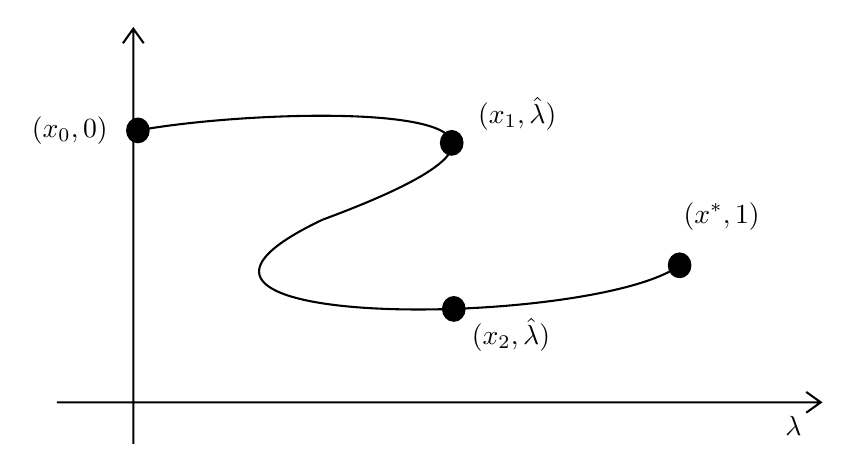
\begin{tikzpicture}[x=0.75pt,y=0.75pt,yscale=-1,xscale=1]
%uncomment if require: \path (0,300); %set diagram left start at 0, and has height of 300

%Curve Lines [id:da9135414320300635] 
\draw    (86.6,88.58) .. controls (129.2,80.84) and (219.29,76.84) .. (235.6,90.58) .. controls (244.57,98.12) and (231.27,111.02) .. (175.6,131.58) ;
%Shape: Axis 2D [id:dp33246942734500173] 
\draw  (47.6,219.58) -- (415.6,219.58)(84.4,39.58) -- (84.4,239.58) (408.6,214.58) -- (415.6,219.58) -- (408.6,224.58) (79.4,46.58) -- (84.4,39.58) -- (89.4,46.58)  ;
%Curve Lines [id:da5784926820320063] 
\draw    (175.6,131.58) .. controls (59.6,186.58) and (307.6,183.58) .. (347.6,153.58) ;
%Flowchart: Connector [id:dp04460202375005207] 
\draw  [fill={rgb, 255:red, 0; green, 0; blue, 0 }  ,fill opacity=1 ] (232.6,94.58) .. controls (232.6,91.43) and (234.93,88.87) .. (237.8,88.87) .. controls (240.68,88.87) and (243,91.43) .. (243,94.58) .. controls (243,97.73) and (240.68,100.29) .. (237.8,100.29) .. controls (234.93,100.29) and (232.6,97.73) .. (232.6,94.58) -- cycle ;
%Flowchart: Connector [id:dp38994047364799467] 
\draw  [fill={rgb, 255:red, 0; green, 0; blue, 0 }  ,fill opacity=1 ] (233.6,174.58) .. controls (233.6,171.43) and (235.93,168.87) .. (238.8,168.87) .. controls (241.68,168.87) and (244,171.43) .. (244,174.58) .. controls (244,177.73) and (241.68,180.29) .. (238.8,180.29) .. controls (235.93,180.29) and (233.6,177.73) .. (233.6,174.58) -- cycle ;
%Flowchart: Connector [id:dp15423490643201487] 
\draw  [fill={rgb, 255:red, 0; green, 0; blue, 0 }  ,fill opacity=1 ] (81.4,88.58) .. controls (81.4,85.43) and (83.73,82.87) .. (86.6,82.87) .. controls (89.47,82.87) and (91.8,85.43) .. (91.8,88.58) .. controls (91.8,91.74) and (89.47,94.29) .. (86.6,94.29) .. controls (83.73,94.29) and (81.4,91.74) .. (81.4,88.58) -- cycle ;
%Flowchart: Connector [id:dp9923370806821367] 
\draw  [fill={rgb, 255:red, 0; green, 0; blue, 0 }  ,fill opacity=1 ] (342.4,153.58) .. controls (342.4,150.43) and (344.73,147.87) .. (347.6,147.87) .. controls (350.47,147.87) and (352.8,150.43) .. (352.8,153.58) .. controls (352.8,156.74) and (350.47,159.29) .. (347.6,159.29) .. controls (344.73,159.29) and (342.4,156.74) .. (342.4,153.58) -- cycle ;

% Text Node
\draw (397,225) node [anchor=north west][inner sep=0.75pt]   [align=left] {$\displaystyle \lambda $};
% Text Node
\draw (249,71) node [anchor=north west][inner sep=0.75pt]   [align=left] {$\displaystyle ( x_{1} ,\hat{\lambda })$};
% Text Node
\draw (246,177.58) node [anchor=north west][inner sep=0.75pt]   [align=left] {$\displaystyle ( x_{2} ,\hat{\lambda })$};
% Text Node
\draw (34,80.4) node [anchor=north west][inner sep=0.75pt]    {$( x_{0} ,0)$};
% Text Node
\draw (348,122) node [anchor=north west][inner sep=0.75pt]   [align=left] {$\displaystyle \left( x^{*} ,1\right)$};
\end{tikzpicture}
\end{figure}

En el ejemplo de la figura, si estamos en una iteración con la estimación $(x_1, \hat{\lambda})$, resulta que $x_1$ no sirve como estimación cercana para resolver $H(x, \lambda+1/N)=0$ porque la curva cambia de sentido.
Nuestro método tendrá que ser más sofisticado para seguir la dirección de la curva aunque eso signifique disminuir $\lambda$ en algún momento.

Obsérvese que la figura ilustra que no podemos parametrizar la solución $x$ respecto $\lambda$ correctamente.
Por ello, a partir de ahora nos referiremos a la curva $c:\mathbb{R}\to\mathbb{R}^{n+1}$ definida por $c(s)=(x(s),\lambda(s))$ que consideraremos parametrizada por longitud de arco y de manera que $H(c(s))=0$ para todo $s \in \mathbb{R}$.
La derivada de $c(s)$ respecto $s$, que escribiremos como $\dot{c}(s)$ y la llamaremos \textbf{tangente} de $c$ en $s$, cumple que:

\begin{enumerate}
	\item $H'(c(s)) \dot{c}(s)=0$
	\item $\|\dot{c}(s)\|=1$ (normalizado)
	\item $det \begin{pmatrix}
		H'(c(s))\\
		\dot{c}(s)^t
	\end{pmatrix}>0$ (orientado positivamente)
\end{enumerate}

Formalizemos que efectivamente podemos parametrizar dicha curva $c(s)$:

\begin{definition}[Punto regular]
	Dada una función $F : \mathbb{R}^n \to \mathbb{R}^p$ con matriz jacobiana $F'$, diremos que un $x\in \mathbb{R}^n$ es un \textbf{punto regular} si $F'(x)$ es una matriz de rango máximo.
\end{definition}

\begin{lemma}
	Dada una función $F : \mathbb{R}^{n+1} \to \mathbb{R}^n$ y un punto regular $x$ de $F$ tal que $F(x)=0$.
	Entonces existe un intervalo $J \subset \mathbb{R}$ y una curva $c: J \to\mathbb{R}^n$ tal que $F(c(s))=0$ para todo $s \in J$.
\end{lemma}
\begin{proof}
	Como $F'(x)$ es matriz $n\times(n+1)$ de rango máximo, podemos quitar una columna y quedarnos con una matriz cuadrada no singular.
	Supongamos si pérdida de generalidad que quitamos la primera columna, corresponiendo con $\frac{\partial F}{\partial x_1}$. 
	Por el teorema de la función inversa, existe un entorno $U$ de $x$ y una función única diferenciable $g : U \to \mathbb{R}^n$ con $g(x_1)=(x_2,\dots,x_n)$ y $F(x_1,g(x_1))$.
	Tomemos ahora la curva $x_1 \mapsto (x_1, g(x_1))$ y reparametrizando, normalizando y orientando dicha curva podemos construir la $c$ del enunciado del lema.
\end{proof}

En particular, para cada punto regular $(x,\lambda)$ de $H$ con $H(x,\lambda)=0$, $H'(x,\lambda)$ define de forma única la curva $c$ normalizada y positivamente orientada que pasa por $(x,\lambda)$ con $c(0)=(x,\lambda)$ y $H(c(s))=0$ para algún intervalo abierto conteniendo el $0$. Usaremos la notación $t(H'(x,\lambda))$ para referirnos a la tangente de dicha curva. 

\begin{definition}[Valor regular]
	Dada una función $F : \mathbb{R}^n \to \mathbb{R}^p$ con matriz jacobiana $F'$, diremos que un $y\in \mathbb{R}^p$ es un \textbf{valor regular} si $F'(x)$ es una matriz de rango máximo para todo $x \in \mathbb{R}^n$ con $F(x)=y$.
	Es decir, $y$ es valor regular si todos los puntos de su preimagen son regulares.
\end{definition}

Estaremos interesados en si el $0 \in \mathbb{R}^n$ es valor regular de la homotopía $H$, pues en ese caso podremos tomar $J=\mathbb{R}$.

\begin{theorem}\label{homotopy-continuation-c-teorema}
	Sea $0$ un valor regular de $H:\mathbb{R}^{n+1}\to\mathbb{R}$. Entonces la curva $c(s)$ está definida en todo $\mathbb{R}$ y satisface una de las dos condiciones siguientes:
	\begin{enumerate}
		\item La curva $c(s)$ es difeomorfa a un círculo. Más precisamente, existe un período $T > 0$, tal que $c(s_1) = c(s_2) \Leftrightarrow s_1 - s_2$ es un entero múltiplo de $T$.
		\item La curva $c(s)$ es difeomorfa a la recta real. Más precisamente, c es inyectiva y $c(s)$ no tiene puntos de acumulación para $s \rightarrow \pm \infty$. 
	\end{enumerate}
\end{theorem}
\begin{proof}
	Podemos describir $c$ como la solución de un problema de valor inicial:
	\begin{enumerate}
		\item $\dot{u} = t(H'(u))$
		\item $u(0) = u_0$
	\end{enumerate}
	Ya que $0$ es un valor regular, ningún cero de $H$ es singular, por tanto $c(s)$ está bien definido en todo $\mathbb{R}$. Como tenemos una EDO autónoma, la solución es invariante por traslación. Vamos a ver lo que ocurre en los siguientes casos:
	\begin{enumerate}
		\item $c$ es no inyectiva. Definimos $T := \min \{ s>0 : c(s) = c(0)\}$. Por unicidad del problema de valor inicial y por la invarianza bajo traslación, tenemos  que la curva $c(s)$ es difeomorfa a un círculo.
		\item $c$ es inyectiva. Veamos que se cumple que la curva $c(s)$ es difeomorfa a la recta real, por reducción al absurdo: \\
		Asumimos sin pérdida de generalidad que $\hat{u}$ es un punto regular de $H$. Usamos el punto inicial $u(0) = \hat{u}$ para definir el problema de valor inicial y obtener una solución $\hat{c}$. Por unicidad, las curvas $c$ y $\hat{c}$ deben ser iguales localmente. Luego existe un $s_1 > 0$ tal que $c(s_1) = \hat{u}$. Como $\hat{u}$ es también un punto de acumulación de $c(s_1 + s)$ cuando $s \longrightarrow \infty$, y como la curva $s \rightarrow c(s_1 + s)$ también es solución, entonces podemos repetir el argumento tomando $s_2 > 0$ tal que $c(s_1 + s_2) = \hat{u}$. Esto contradice la inyectividad de c.
	\end{enumerate}
\end{proof}

\section{Método de continuación de Euler-Newton}

Sea $A$ una matriz $n\times(n+1)$ de rango máximo. Al no ser una matriz cuadrada, no podemos obtener su inversa. Sin embargo, se conoce de álgebra lineal que como $A$ es una matriz real, su rango coincide con el rango de $AA^t$. Por lo tanto, $AA^t$ es una matriz cuadrada $n\times n$ de rango $n$, luego es invertible. Esto motiva la siguiente definición: 

\begin{definition}
	Sea $A$ una matriz $n\times(n+1)$ de rango máximo. La \textbf{inversa de Moore-Penrose} de $A$ es una matriz $A^+$ definida por $A^+=A^t(AA^t)^{-1}$.
\end{definition}

Obsérvese que $AA^+=(AA^t)(AA^t)^{-1}=A$, por lo que $A^+$ es una inversa derecha de $A$.

A continuación, veremos el método de continuación de Euler-Newton. Es un método predictor-corrector, es decir, que en cada iteración realiza toma una estimación aproximada que luego corrige con el método de Newton.

\begin{algorithm}[H]
	\floatname{algorithm}{Algoritmo}
	\caption{Método de Euler-Newton Predictor-Corrector}
	\textbf{Entrada: } \\
	\hspace*{\algorithmicindent} $H$ \text{ - homotopía de una función $G(x)$ a $F(x)$} \\
	\hspace*{\algorithmicindent} $x_0$ \text{ - cero de $H(x,0)=G(x)$} \\
	%\hspace*{\algorithmicindent} $TOL$ \text { - tolerancia} \\
	\hspace*{\algorithmicindent} $N$ \text{ - número máximo de iteraciones de predicción} \\
	\hspace*{\algorithmicindent} $M$ \text{ - número máximo de iteraciones de corrección} \\
	\textbf{Salida:} \\
	\hspace*{\algorithmicindent} $x$ \text{ - cero aproximado de } $F$
	\begin{algorithmic}
		\Procedure {}{}
		\State $h = \frac{1}{N}$ \Comment{Paso}
		\State $u = (x,0)$
		\For{$k = 1,\dots,N$}
			\State $v = u + ht(H'(u))$ \Comment{Predicción}
			\For{$j = 1,\dots,M$} \Comment{Corrección}
				\State $v = v - H'(v)^+H(v)$
				\State \textbf{salir del bucle si converge}
			\EndFor
			\State $u = v$
			\State \textbf{salir del bucle si converge}
		\EndFor
		$(x, \lambda) = u$
		\State \Return x \Comment{Solución obtenida}
		\EndProcedure
	\end{algorithmic}
\end{algorithm}

Obsérvese que la corrección es muy similar al método de Newton. La idea de la corrección se presenta en la siguiente figura.

\begin{figure}[H]
	\centering

	\tikzset{every picture/.style={line width=0.75pt}} %set default line width to 0.75pt        

	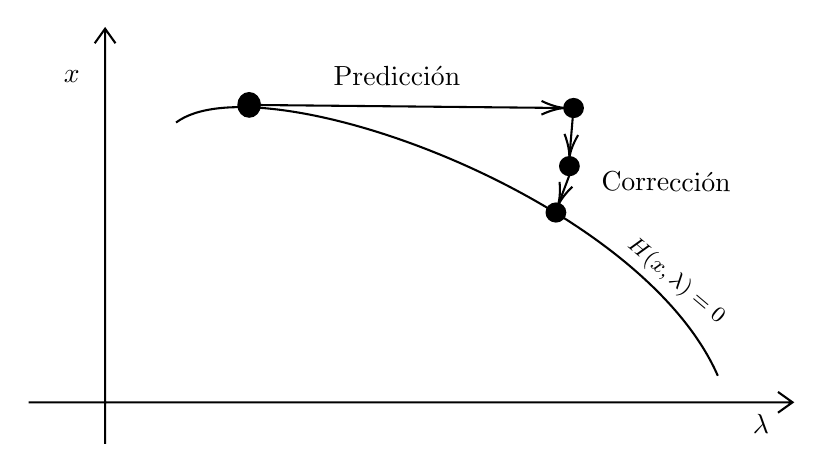
\begin{tikzpicture}[x=0.75pt,y=0.75pt,yscale=-1,xscale=1]
	%uncomment if require: \path (0,300); %set diagram left start at 0, and has height of 300
	
	%Curve Lines [id:da3653140690727089] 
	\draw    (102.6,130.78) .. controls (142.6,100.78) and (325.6,165.78) .. (363.6,252.78) ;
	%Flowchart: Connector [id:dp392125415090699] 
	\draw  [fill={rgb, 255:red, 0; green, 0; blue, 0 }  ,fill opacity=1 ] (132.6,122.29) .. controls (132.6,119.13) and (134.93,116.58) .. (137.8,116.58) .. controls (140.68,116.58) and (143,119.13) .. (143,122.29) .. controls (143,125.44) and (140.68,127.99) .. (137.8,127.99) .. controls (134.93,127.99) and (132.6,125.44) .. (132.6,122.29) -- cycle ;
	%Straight Lines [id:da32974900830101495] 
	\draw    (137.8,122.29) -- (215.6,123.05) -- (287.6,123.76) ;
	\draw [shift={(289.6,123.78)}, rotate = 180.57] [color={rgb, 255:red, 0; green, 0; blue, 0 }  ][line width=0.75]    (10.93,-3.29) .. controls (6.95,-1.4) and (3.31,-0.3) .. (0,0) .. controls (3.31,0.3) and (6.95,1.4) .. (10.93,3.29)   ;
	%Flowchart: Connector [id:dp396415556899567] 
	\draw  [fill={rgb, 255:red, 0; green, 0; blue, 0 }  ,fill opacity=1 ] (289.6,123.78) .. controls (289.6,121.38) and (291.61,119.43) .. (294.1,119.43) .. controls (296.59,119.43) and (298.6,121.38) .. (298.6,123.78) .. controls (298.6,126.19) and (296.59,128.14) .. (294.1,128.14) .. controls (291.61,128.14) and (289.6,126.19) .. (289.6,123.78) -- cycle ;
	%Flowchart: Connector [id:dp8330801591176681] 
	\draw  [fill={rgb, 255:red, 0; green, 0; blue, 0 }  ,fill opacity=1 ] (287.6,151.78) .. controls (287.6,149.38) and (289.61,147.43) .. (292.1,147.43) .. controls (294.59,147.43) and (296.6,149.38) .. (296.6,151.78) .. controls (296.6,154.19) and (294.59,156.14) .. (292.1,156.14) .. controls (289.61,156.14) and (287.6,154.19) .. (287.6,151.78) -- cycle ;
	%Flowchart: Connector [id:dp25418827796224785] 
	\draw  [fill={rgb, 255:red, 0; green, 0; blue, 0 }  ,fill opacity=1 ] (281.1,174.14) .. controls (281.1,171.73) and (283.11,169.78) .. (285.6,169.78) .. controls (288.09,169.78) and (290.1,171.73) .. (290.1,174.14) .. controls (290.1,176.54) and (288.09,178.49) .. (285.6,178.49) .. controls (283.11,178.49) and (281.1,176.54) .. (281.1,174.14) -- cycle ;
	%Straight Lines [id:da9516946974155029] 
	\draw    (294.1,123.78) -- (293.08,135.82) -- (292.27,145.44) ;
	\draw [shift={(292.1,147.43)}, rotate = 274.83] [color={rgb, 255:red, 0; green, 0; blue, 0 }  ][line width=0.75]    (10.93,-3.29) .. controls (6.95,-1.4) and (3.31,-0.3) .. (0,0) .. controls (3.31,0.3) and (6.95,1.4) .. (10.93,3.29)   ;
	%Straight Lines [id:da17213986288020022] 
	\draw    (292.1,156.14) -- (287.3,168.91) ;
	\draw [shift={(286.6,170.78)}, rotate = 290.58] [color={rgb, 255:red, 0; green, 0; blue, 0 }  ][line width=0.75]    (10.93,-3.29) .. controls (6.95,-1.4) and (3.31,-0.3) .. (0,0) .. controls (3.31,0.3) and (6.95,1.4) .. (10.93,3.29)   ;
	%Shape: Axis 2D [id:dp7268441229557736] 
	\draw  (31.6,265.58) -- (399.6,265.58)(68.4,85.58) -- (68.4,285.58) (392.6,260.58) -- (399.6,265.58) -- (392.6,270.58) (63.4,92.58) -- (68.4,85.58) -- (73.4,92.58)  ;
	
	% Text Node
	\draw (177,102) node [anchor=north west][inner sep=0.75pt]   [align=left] {Predicción};
	% Text Node
	\draw (306.13,152.56) node [anchor=north west][inner sep=0.75pt]  [rotate=-0.88] [align=left] {Corrección};
	% Text Node
	\draw (379,270) node [anchor=north west][inner sep=0.75pt]   [align=left] {$\displaystyle \lambda $};
	% Text Node
	\draw (47,104.4) node [anchor=north west][inner sep=0.75pt]    {$x$};
	% Text Node
	\draw (324.66,182.45) node [anchor=north west][inner sep=0.75pt]  [font=\footnotesize,rotate=-40.12]  {$H( x,\lambda ) =0$};
	
	\end{tikzpicture}	
\end{figure}

Ahora veamos la implementación del algoritmo en SAGE:

\begin{minted}{python}
def tangente(A):
	A = matrix(CDF, A)
	Q, R = A.transpose().QR()
	tang = Q.columns()[-1]
	signo = Q.determinant() * R[:-1,:].determinant()
	return tang  
	
def invMoorePenrose(A):
	return A.transpose()*(A*A.transpose()).inverse()
	
def var_subs(variables, values):
	return {str(va): ui for va, ui in zip(variables, values)}
	
def EulerNewtonContinuacionHomotopica(H, variables, x0=None, eps=0.001, N=20, M=20):
	J = jacobian(H, variables)
	h = 1/N
	if x0 is None:
	x0 = (random() for _ in variables[:-1])
	u0 = vector((*x0, 0))
	uk = [u0]
	prediction = [u0]
	for k in [1..N]:
		u = uk[k-1]
		if u[-1]+eps > 1:
			break
	v = u + h*tangente(J(**var_subs(variables, u)))
	prediction.append(v)
	for j in [1..M]:
		correction = invMoorePenrose(J(**var_subs(variables, v)))
						*H(**var_subs(variables, v))
		if correction.norm() < eps:
			break
	v = v - correction
	uk.append(v)
	return uk
\end{minted}

\section{Homotopía de Newton}
El último ingrediente que nos falta es la homotopía $H$ en sí. Sea $a\in\mathbb{R}^n$ un punto cualquiera. Definimos entonces la homotopía $H:\mathbb{R}^n\times [0,1] \to \mathbb{R}^n$ por:
\[ H(x,\lambda) = \lambda F(x) + (1- \lambda) [F(x)- F(a)] = F(x) - (1-\lambda) F(a) \]

Claramente, $H \in \mathcal{C}^\infty$. Además, tenemos que una solución de $H(x,0)=F(x)-F(a)$ es $x=a$. Por lo tanto, a partir de ahora, diremos $x(0)$ para referirnos a $a$.
Para esta $H$ la ecuación $H(x,\lambda)=0$ toma la forma:

\[ F(x) = (1 - \lambda) F(a) \]

Sea $\Omega \subseteq \mathbb{R}^n$ un abierto acotado tal que su borde $\delta \Omega$ es una suave (entendido como una subvariedad $\mathcal{C}^\infty$) y conexa.
Para saber si el cero es un valor regular de $H$ nos basaremos en las siguientes condiciones:

\begin{definition}[Condiciones de Smale]
	\begin{itemize}
		\item[]
		\item $0$ es un valor regular de $F$.
		\item $F(x) \neq 0$ para todo $x\in\delta\Omega$.
		\item $F'(x)$ es no singular para todo $x\in\delta\Omega$.
		\item Para todo $x\in\delta\Omega$, la dirección $-(F'(x))^{-1}F(x)$ no es tangente a $\delta\Omega$.
	\end{itemize}
\end{definition}

Peter Percell demostró que dichas condiciones implican que el cero es valor regular de $H$ para casi toda elección de $a$. 

%%%%%%%%%%%%%%%%%%%%%%%%%%%%%%%%%%%%%%%%%%%%%%%%%%%%%%%%%%%%%%%%%
%(11.4.8) Theorem. [Smale (1976) 
\begin{theorem}
	Sea $\Omega \subset \mathbb{R}^n$ un abierto acotado con borde suave y sea $F: \mathbb{R}^n \longrightarrow \mathbb{R}^n$. Supongamos que $F \in \mathcal{C}^\infty$ y se cumplen las condiciones de Smale. Elijamos un $a \in \partial \Omega$ cumpliendo que $0$ es un valor regular de la correspondiente homotopía de Newton $H$. Sea $c_a$ la curva parametrizada por longitud de arco dada por el teorema \ref{homotopy-continuation-c-teorema} tal que:
	\begin{enumerate}
		\item $x(0) = a$, $\lambda(0) = 0$.
		\item $\dot{x}(0)$ apunta dentro de $\Omega$.
	\end{enumerate}
	Entonces hay un parámetro $s_0 > 0$ tal que:
	\begin{enumerate}
		\item[3.] $x(s) \in \Omega$ para todo $s \in (0,s_0)$.
		\item[4.] $x(s_0) \in \partial \Omega$.
		\item[5.] $\lambda(s_0) > 1$.
	\end{enumerate}
	En consecuencia, la curva $c_a$ se cruza al objetivo al nivel $\{1\}\times\Omega$ en un número impar de puntos $(1,\hat{x}) \in \{1\}\times\Omega$, donde $F(\hat{x}) = 0$.
\end{theorem}
\begin{proof}
	Como $\partial \Omega$ es conexa, asumimos sin pérdida de generalidad que la dirección de Newton $-(F'(x))^{-1}F(x)$ siempre apunta hacia $\Omega$ para $x \in \partial \Omega$. De no ser así, simplemente cambiamos los signos y volvemos a empezar. Derivamos la ecuación homotópica $F(x(s)) - (1-\lambda(s)) F(a)=0$ respecto $s$.
	\[ F'(x(s)) \dot{x}(s) - (1-\dot{\lambda}(s))F(a) \]
	Sustituyendo $(1-\lambda(s))^{-1}F(x(s))$ por $F(a)$ obtenemos que si $\lambda(s) \neq 1$:
	\[ F'(x(s)) \dot{x}(s) - \frac{1-\dot{\lambda}(s)}{1-\lambda(s)} F(x(s)) = 0 \]
	
	Tomando $s=0$ y multiplicando por $(F'(a))^{-1}$, la ecuación anterior se transforma en:
	\[ \dot{x}(0) - (1-\dot{\lambda}(0)) (F'(a))^{-1}F(a) = 0 \]
	Ahora bien, como $\dot{x}(0)$ y $-(F'(a))^{-1}F(a)$ apuntan hacia dentro de $\Omega$, para que su suma se anule es necesario que $1-\dot{\lambda}(0)<0$.
	
	Ya que $F(a) \neq 0$ y $\Omega$ está acotada, entonces el conjunto $\{\lambda : F(x) = (1-\lambda) F(a) , x \in \overline{\Omega}\}$ está también acotado.
	Entonces la curva $\mathcal{C}_a$ debe salirde $\mathbb{R} \times \Omega$ para cierto parámetro $s_0 >  0$.
	Veamos que $1-\lambda(s_{0}) < 0$:

	Como $\dot{x}(s_{0})$ apunta hacia fuera de $\Omega$, siguiendo un razonamiento similar para el caso $s=0$, se puede deducir que $\frac{1-\dot{\lambda}(s_{0})}{1-\lambda(s_{0})} > 0$. Ahora consideremos el Jacobiando aumentado:
	\begin{equation*}
		A(s) :=
		\begin{pmatrix}
			F'(x(s)) & -G(a) \\
			\dot{x}(s)^t & \dot{\lambda}(s)
		\end{pmatrix}
	\end{equation*}
de la homotopía $H$. Entonces obtendremos que:
	\begin{equation*}
		A(s)
		\begin{pmatrix}
			Id & \dot{x}(s) \\
			0^* & \dot{\lambda}(s)
		\end{pmatrix}
		=
		\begin{pmatrix}
			F'(x(s)) & 0 \\
			\dot{x}(s)^* & 1
		\end{pmatrix}
	\end{equation*}
y consecuentemente $\det A(s) \dot{\lambda}(s) = \det F'(x(s))$.
Como el jacobiano $F'(a)$ es no singular para $a \in \partial \Omega$, y siendo que $\partial \Omega$ es conexa, la función $F'(x)$ no cambia de signo en $\partial \Omega$.
Por otro lado, la función $\det A(s)$ no cambia de signo a lo largo del $c_{a}$.
En consecuencia, como $1-\dot{\lambda} < 0$ y por lo anterior obtenido, $1-\dot{\lambda}(s_{0}) < 0$.
Como $\frac{1-\dot{\lambda}(s_{0})}{1-\lambda(s_{0})} > 0$, entonces obtenemos que $1-\lambda(s_{0}) < 0$.
Así pues, como $\lambda(0) < 1$ y $\lambda(s_0)$ debe haber una cantidad impar de soluciones de $\lambda(s)=1$ para $s \in (0,1)$. 
\end{proof}

Ilustramos en la siguiente figura un ejemplo en el que se encuentran tres soluciones, los tres puntos donde la curva corta con el plano $\Omega \times \{1\}$.

\begin{figure}[H]
\centering 
\tikzset{every picture/.style={line width=0.75pt}} %set default line width to 0.75pt        

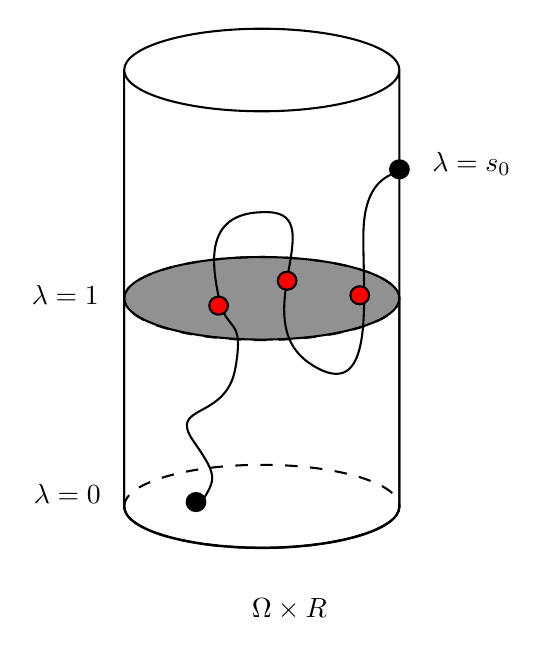
\begin{tikzpicture}[x=0.75pt,y=0.75pt,yscale=-1,xscale=1]
%uncomment if require: \path (0,320); %set diagram left start at 0, and has height of 320

%Shape: Can [id:dp7299935234454771] 
\draw   (372.6,30.27) -- (372.6,240.49) .. controls (372.6,251.48) and (342.92,260.38) .. (306.3,260.38) .. controls (269.68,260.38) and (240,251.48) .. (240,240.49) -- (240,30.27) .. controls (240,19.29) and (269.68,10.38) .. (306.3,10.38) .. controls (342.92,10.38) and (372.6,19.29) .. (372.6,30.27) .. controls (372.6,41.26) and (342.92,50.16) .. (306.3,50.16) .. controls (269.68,50.16) and (240,41.26) .. (240,30.27) ;
%Shape: Can [id:dp47125227248383883] 
\draw   (372.6,140.27) -- (372.6,240.69) .. controls (372.6,251.68) and (342.92,260.58) .. (306.3,260.58) .. controls (269.68,260.58) and (240,251.68) .. (240,240.69) -- (240,140.27) .. controls (240,129.29) and (269.68,120.38) .. (306.3,120.38) .. controls (342.92,120.38) and (372.6,129.29) .. (372.6,140.27) .. controls (372.6,151.26) and (342.92,160.16) .. (306.3,160.16) .. controls (269.68,160.16) and (240,151.26) .. (240,140.27) ;
%Shape: Ellipse [id:dp3528139206176152] 
\draw  [dash pattern={on 4.5pt off 4.5pt}] (240,240.49) .. controls (240,229.45) and (269.68,220.49) .. (306.3,220.49) .. controls (342.92,220.49) and (372.6,229.45) .. (372.6,240.49) .. controls (372.6,251.54) and (342.92,260.49) .. (306.3,260.49) .. controls (269.68,260.49) and (240,251.54) .. (240,240.49) -- cycle ;
%Curve Lines [id:da020871625686910256] 
\draw    (274.6,242.78) .. controls (283.97,227.33) and (286.37,227.72) .. (273.48,209.25) .. controls (260.6,190.78) and (289.19,199.55) .. (293.6,173.78) .. controls (298.01,148.02) and (289.39,158.11) .. (285.49,139.45) .. controls (281.6,120.78) and (279.6,97.78) .. (309.6,98.78) .. controls (339.6,99.78) and (298.03,151.06) .. (329.82,171.92) .. controls (361.6,192.78) and (354.92,140.12) .. (355.23,109.57) .. controls (355.54,79.02) and (372.37,81.26) .. (372.6,78.14) ;
%Shape: Ellipse [id:dp31954427248086303] 
\draw  [fill={rgb, 255:red, 0; green, 0; blue, 0 }  ,fill opacity=0.43 ][dash pattern={on 4.5pt off 4.5pt}] (240,140.38) .. controls (240,129.34) and (269.68,120.38) .. (306.3,120.38) .. controls (342.92,120.38) and (372.6,129.34) .. (372.6,140.38) .. controls (372.6,151.43) and (342.92,160.38) .. (306.3,160.38) .. controls (269.68,160.38) and (240,151.43) .. (240,140.38) -- cycle ;
%Flowchart: Connector [id:dp040262084755504635] 
\draw  [fill={rgb, 255:red, 255; green, 0; blue, 0 }  ,fill opacity=1 ] (280.99,143.8) .. controls (280.99,141.4) and (283.01,139.45) .. (285.49,139.45) .. controls (287.98,139.45) and (289.99,141.4) .. (289.99,143.8) .. controls (289.99,146.21) and (287.98,148.16) .. (285.49,148.16) .. controls (283.01,148.16) and (280.99,146.21) .. (280.99,143.8) -- cycle ;
%Flowchart: Connector [id:dp9468422676368585] 
\draw  [fill={rgb, 255:red, 255; green, 0; blue, 0 }  ,fill opacity=1 ] (313.99,131.8) .. controls (313.99,129.4) and (316.01,127.45) .. (318.49,127.45) .. controls (320.98,127.45) and (322.99,129.4) .. (322.99,131.8) .. controls (322.99,134.21) and (320.98,136.16) .. (318.49,136.16) .. controls (316.01,136.16) and (313.99,134.21) .. (313.99,131.8) -- cycle ;
%Flowchart: Connector [id:dp18087920406140756] 
\draw  [fill={rgb, 255:red, 255; green, 0; blue, 0 }  ,fill opacity=1 ] (348.99,138.8) .. controls (348.99,136.4) and (351.01,134.45) .. (353.49,134.45) .. controls (355.98,134.45) and (357.99,136.4) .. (357.99,138.8) .. controls (357.99,141.21) and (355.98,143.16) .. (353.49,143.16) .. controls (351.01,143.16) and (348.99,141.21) .. (348.99,138.8) -- cycle ;
%Flowchart: Connector [id:dp7631966333705258] 
\draw  [fill={rgb, 255:red, 0; green, 0; blue, 0 }  ,fill opacity=1 ] (368.1,78.14) .. controls (368.1,75.73) and (370.11,73.78) .. (372.6,73.78) .. controls (375.09,73.78) and (377.1,75.73) .. (377.1,78.14) .. controls (377.1,80.54) and (375.09,82.49) .. (372.6,82.49) .. controls (370.11,82.49) and (368.1,80.54) .. (368.1,78.14) -- cycle ;
%Flowchart: Connector [id:dp3302821570711616] 
\draw  [fill={rgb, 255:red, 0; green, 0; blue, 0 }  ,fill opacity=1 ] (270.1,238.43) .. controls (270.1,236.02) and (272.11,234.08) .. (274.6,234.08) .. controls (277.09,234.08) and (279.1,236.02) .. (279.1,238.43) .. controls (279.1,240.83) and (277.09,242.78) .. (274.6,242.78) .. controls (272.11,242.78) and (270.1,240.83) .. (270.1,238.43) -- cycle ;

% Text Node
\draw (194,132.4) node [anchor=north west][inner sep=0.75pt]    {$\lambda =1$};
% Text Node
\draw (195,228.4) node [anchor=north west][inner sep=0.75pt]    {$\lambda =0$};
% Text Node
\draw (300,283.4) node [anchor=north west][inner sep=0.75pt]    {$\Omega \times \mathbb{R}$};
% Text Node
\draw (387,68.4) node [anchor=north west][inner sep=0.75pt]    {$\lambda =s_{0}$};


\end{tikzpicture}
\end{figure}

\begin{comment}
\begin{theorem}[Factibilidad del método de continuación]
	Sea $F(x) \in \mathcal{C}^{1}$ para $x \in \mathbb{R}^n$. Si la matriz Jacobiana J es no singular para todo $x \in \mathbb{R}^n$, y $\exists M : ||J(x)^{-1}|| \leq M$, $\forall x \in \mathbb{R}^n$. Entonces: 
	\[\forall x(0) \in \mathbb{R}^n, \; \exists x(\lambda) : H(x(\lambda),\lambda) = 0\]
	Es decir, si J es no singular y su inversa es acotada, entonces encontraremos solución para cualquier valor inicial que tomemos.
\end{theorem}

	Para esta demostración, vamos a hacer uso del teorema de la función implícita y de las aplicaciones ofrecidas por Milnor (1969). Además, los métodos de embebimiento visto por Ficker (1951), Wasserstrom (1973) y Wacker (1978).
\begin{proof}
	Definimos una curva implícita $c(s) \in H^{-1}(0)$ desde el punto inicial $(0,x_0)$ hasta la solución $(1,\hat{x})$.
	Por el teorema de la función implícita, si el Jacobiano $H'(0,x_0)$ tiene rango máximo, entonces la curva $c(s) \in H^{-1}(0)$ con punto inicial $c(0) = (0,x_0)$ y tangente $c(0) \neq 0$ existe al menos localmente. Es decir, existe al menos en un intervalo alrededor del cero.\\
	Por otro lado, si todos los ceros de $H$ son valores regulares, entonces la curva $c(s)$ es un difeomorfismo de la recta real o de un círculo. Es decir, que dicha curva existe.\\
	Para ver que en una distancia finita la curva se cruza con $\lambda = 1$, de forma que se obtiene la solución, tenemos que usar los teoremas de existencia para análisis no lineal. Es suficiente con exigir que la inversa esté acotada para que la curva no se vaya al infinito antes de intersectar $\lambda = 1$ o antes de volver a $\lambda = 0$. Los problemas de acotación serán estudiados uno por uno. \\
	Por último, para parametrizar dicha curva utilizaremos los métodos de embebimiento.
\end{proof}
\end{comment}

\begin{example}
	
	Vamos a tomar el ejemplo comparativo que hemos usado hasta ahora:
	
	\begin{align*}
		f_1(x,y,z) &= 3x - cos(yz) - \frac{1}{2} \\
		f_2(x,y,z) &= x^2 - 81(y+0.1)^2 + sin(z) + 1.06\\
		f_3(x,y,z) &= exp(-xy) + 20z + \frac{10\pi-3}{3}
	\end{align*}
	
	Denotamos $F(x,y,z) = (f_1(x,y,z),f_2(x,y,z),f_3(x,y,z))$.
	Aplicamos el algoritmo de continuación de Euler-Newton a la función $H(x,y,z,t) = F(x,y,z)-(1-t)F(x_0)$, de variables $(x,y,z,t)$, en el punto inicial $x_0 = (0.1,0.1,-0.1)$.
	Obtenemos la solución aproximada $(0.50457,-0.00072,-0.52841,1.01144)$.
\end{example}

\begin{example}
	Tomemos la función $f(x) = cos(x)-x$ y el punto inicial $x_0 = 0$. Entonces nuestra función $H(x,t) = f(x)-(1-t)f(x_0)$. Aplicando nuestro algoritmo a $H$ y obtenemos la solución $(0.74157,1.00239)$.
	
	Observamos gráficamente:\\
	
	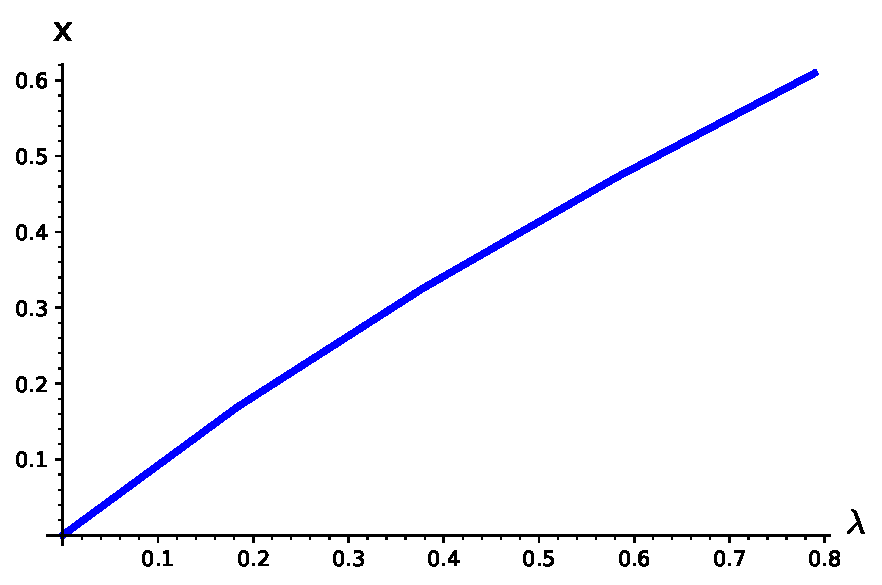
\includegraphics[scale=0.5]{imagenes/ejemplo1_continuacion.pdf}{\centering}
	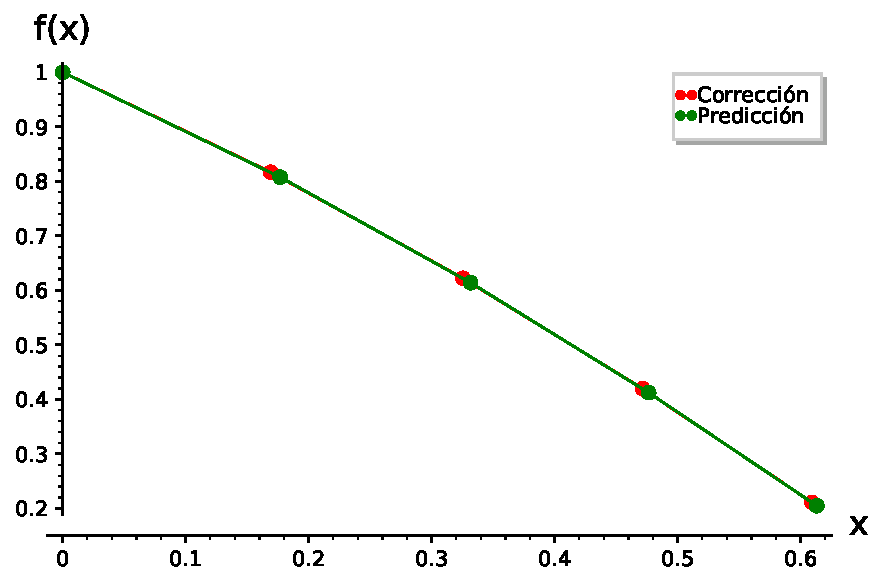
\includegraphics[scale=0.5]{imagenes/ejemplo1_1_continuacion.pdf}{\centering}\\
	Para que se aprecie la diferencia entre la predicción y la corrección, hemos tomado tan solo 4 pasos.

\end{example}

\begin{example}
	Tomemos la función $f(x) = x^2$ y el punto inicial $x_0 = 0.2$. Entonces nuestra función $H(x,t) = f(x)-(1-t)f(x_0)$. Aplicando nuestro algoritmo a $H$ y obtenemos la solución $(-0.00584,0.99980)$.
	
	Observamos gráficamente:\\
	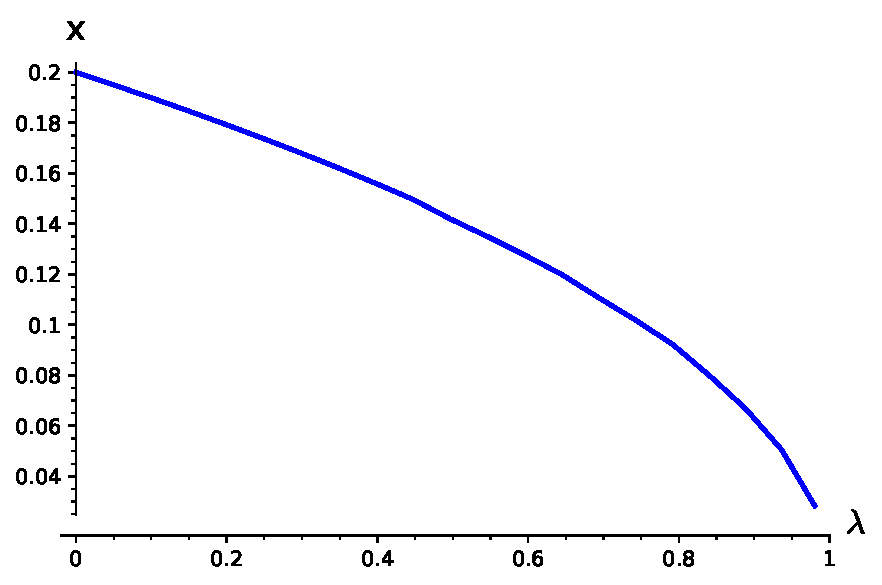
\includegraphics[scale=0.5]{imagenes/ejemplo2_continuacion.pdf}{\centering}
	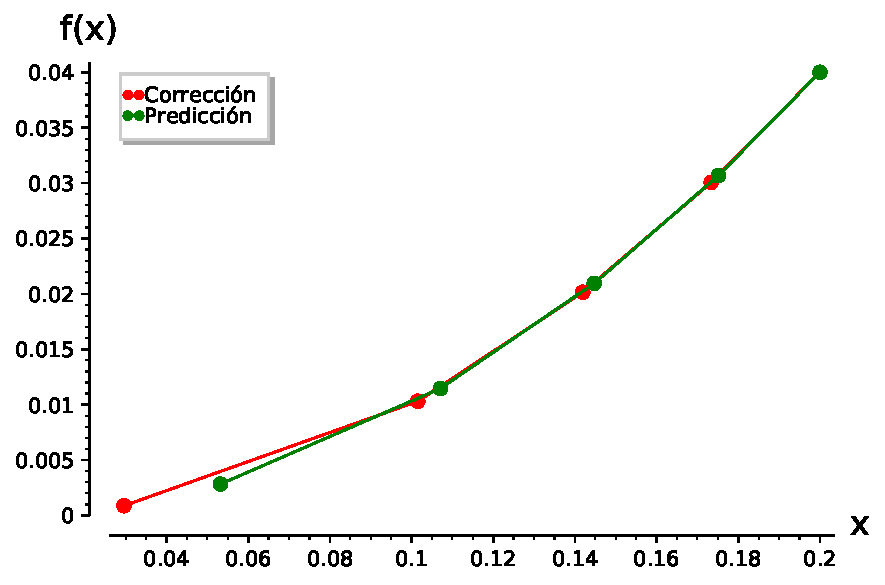
\includegraphics[scale=0.5]{imagenes/ejemplo2_1_continuacion.pdf}{\centering}
	
\end{example}


\section{Métodos y software}


Hemos considerados métodos para aproximar soluciones de sistemas de ecuaciones no lineales. Hemos visto que el método de Newton requiere de una buena aproximación inicial para funcionar, pero que converge rápidamente a la solución. Sin embargo, también requiere resolver un problema de orden $O(n^3)$ computacionalmente.\\

El método de Broyden reduce la cantidad de cálculos sin comprometer demasiado la rapidez de convergencia, usando como técnica un reemplazamiento de la matriz Jacobiana por una matriz cuya inversa es determinada en cada paso. Así reducimos la carga computacional a $O(n^2)$. Por otro lado, este método también requiere una buena aproximación inicial. \\

El método de máximo descenso presenta una forma de obtener una buena aproximación inicial, pero a cambio no nos da una rápida convergencia. \\

Los métodos de homotopía y continuación también pueden aplicarse a sistemas no lineales. El paquete Homepack de Netlib puede resolver sistemas de ecuaciones no lineales mediante el método de homotopía. \\

Los sistemas no lineales usados en librerías IMSL y en NAG usan el método de sistemas no lineales se basan en dos subrutinas IBRD y HYBRJ, contenidas en MINPACK, que es un paquete de dominio público. Ambos utilizan el método de Levenberg-Marquardt, que se trata de un promedio ponderado entre el Método de Newton y el Método de Máximo Descenso. Antes de probar la convergencia utiliza el Método de Máximo Descenso, y luego cambia al método de Newton para conseguir una convergencia más rápida. \\

La subrutina HYBRD emplea una aproximación de diferencias finitas a la matriz Jacobiana. Con la subrutina NEQNF de IMSL se resuelve un sistema no lineal sin necesidad de introducir nosotros la matriz Jacobiana. \\

En la librería NAG, CO5NBF es parecida a HYBRD. Su subrutina será introduciendo la matriz Jacobiana. Ésta se basa en HYBRJ del paquete de MINPACK. NAH también contiene otra modificación del método de Levenberg-Marquardt.\\

Un tratamiento exhaustivo de los métodos de sistemas no lineales lo encontramos en Ortega y Rheinbolt, y en Dennis y Schnabel. Los avances más recientes se explican en Argyros y Szidarovsky. Para los métodos continuos podemos consultar Allgower y Georg.


%%%%%%%%%%%%%%%%%%%%%%%%%%%%%%%%%%%%%%%%%%%%%%%%%%%%%%

%\begin{lemma}\ref{lambek-lemma}
%\end{lemma}


%\begin{minted}{haskell}

%\end{minted}

%\begin{example}

%\end{example}


